\documentclass{article}
\usepackage[french,english]{babel}
\usepackage[margin=1.2in]{geometry}
\usepackage[utf8]{inputenc}
\usepackage{amssymb}
\usepackage{mathtools}
\usepackage{array}
\usepackage{graphicx} 
\usepackage{color}
\usepackage[usenames,dvipsnames]{xcolor}
\usepackage[T1]{fontenc}
\usepackage{listings}
\usepackage{courier}
\usepackage{caption}
\usepackage{subcaption}

\title{RapportSupelec_TravelJournal}
\setcounter{secnumdepth}{3}
\definecolor{bluekeywords}{rgb}{0.13,0.13,1}
\definecolor{greencomments}{rgb}{0,0.5,0}
\definecolor{redstrings}{rgb}{0.9,0,0}
\lstset{
	language=[Sharp]C,
         basicstyle=\footnotesize\ttfamily, % Standardschrift
         %numbers=left,               % Ort der Zeilennummern
         numberstyle=\tiny,          % Stil der Zeilennummern
         %stepnumber=2,               % Abstand zwischen den Zeilennummern
         numbersep=5pt,              % Abstand der Nummern zum Text
         tabsize=2,                  % Groesse von Tabs
         commentstyle=\color{greencomments},
         stringstyle=\color{redstrings},
         extendedchars=true,         %
         breaklines=true,            % Zeilen werden Umgebrochen
         keywordstyle=\color{bluekeywords}\bfseries,
    		frame=b,         
 %        keywordstyle=[1]\textbf,    % Stil der Keywords
 %        keywordstyle=[2]\textbf,    %
 %        keywordstyle=[3]\textbf,    %
 %        keywordstyle=[4]\textbf,   \sqrt{\sqrt{}} %
         showspaces=false,           % Leerzeichen anzeigen ?
         showtabs=false,             % Tabs anzeigen ?
         xleftmargin=17pt,
         framexleftmargin=17pt,
         framexrightmargin=5pt,
         framexbottommargin=4pt,
         morecomment=[s][\color{javadocblue}]{/**}{*/},
         escapeinside=\`\`,
         %backgroundcolor=\color{lightgray},
         showstringspaces=false      % Leerzeichen in Strings anzeigen ?        
}

    %\DeclareCaptionFont{blue}{\color{blue}} 

  %\captionsetup[lstlisting]{singlelinecheck=false, labelfont={blue}, textfont={blue}}
\usepackage{caption}
\DeclareCaptionFont{white}{\color{white}}
\DeclareCaptionFormat{listing}{\colorbox[cmyk]{0.43, 0.35, 0.35,0.01}{\parbox{\textwidth}{\hspace{15pt}#1#2#3}}}
\captionsetup[lstlisting]{format=listing,labelfont=white,textfont=white, singlelinecheck=false, margin=0pt, font={bf,footnotesize}}


\begin{document}
\selectlanguage{french}

\newcommand\highlight[1]{\colorbox{yellow}{#1}} 
\renewcommand\thesection{\arabic{section}}
\begin{titlepage}
\newcommand{\HRule}{\rule{\linewidth}{1mm}} % Defines a new command for the horizontal lines, change thickness here
\newcommand{\VRule}{\rule{\lineheight}{0.2mm}} % Defines a new command for the vertical lines, change thickness here
\center % Center everything on the page

%----------------------------------------------------------------------------------------
% TITLE >> HEADING SECTIONS
%----------------------------------------------------------------------------------------
\begin{figure}[h ]
\centering

\includegraphics[width=50mm]{Logo_Supelec_RVB.jpg}
\end{figure}
\textsc{\LARGE Supelec - campus de metz}\\[0.5cm] % Minor heading such as course title
%----------------------------------------------------------------------------------------
% TITLE >> TITLE SECTION
%----------------------------------------------------------------------------------------
\vspace{1.2cm}
\HRule \\[0.5cm]
{\textsc{\Huge \bfseries Projet de conception}\\[1cm]{\huge Developpement d'une application Windows Phone 8 pour générer les albums de voyage dynamiquement  \bfseries }}\\[0.4cm] 
\HRule \\[1.5cm]
%----------------------------------------------------------------------------------------
% TITLE >> AUTHOR SECTION
%----------------------------------------------------------------------------------------
\vspace{2.5cm}
\Large {
Promo 2015\\ 
\vspace{1cm}
Hao\ \textsc{XIONG} \ \ \ \
Min\ \textsc{ZHAO}
}
%----------------------------------------------------------------------------------------
\vfill % Fill the rest of the page with whitespace
\end{titlepage}
%----------------------------------------------------------------------------------------
% TITLE >> END
%----------------------------------------------------------------------------------------
\tableofcontents 
\newpage
\listoffigures 
\newpage
\lstlistoflistings
\newpage

%----------------------------------------------------------------------------------------
% PRESECTION
%----------------------------------------------------------------------------------------
\vspace{2cm}
\section{\LARGE INTRODUCTION}


Aujourd’hui c’est une ère de l’information, les gens possèdent des dispositifs de types différents plus abondants par rapport au précédent. L’émergence du terminal mobile nous apporte des diverses facilités et conforts. Les applications mobiles jouent un rôle très important dans ce processus-là. 
\\\\
Apparemment, les caméras de mobile deviennent de plus évolués et pratiques. Il existe pas mal des applications de photo et de l’image, mais les manières qu’ils ont utilisés pour traiter ou organiser des photos ne sont pas assez riches et amusants. En effet, les applications de ce type n’ont pas été beaucoup évoluées depuis les années. A notre avis, nous pouvons développer une (ou plusieurs) visualisation plus dynamique et intéressante en bénéficiant des informations des photos, du temps, d’emplacement, etc.
\\\\
C’est la raison pour laquelle nous avons décidé de réaliser une application pour visualiser les photos dans notre projet de cette année. Plus concrètement, c’est une application pour générer un album de voyage dynamiquement.  Pour bien dérouler notre projet, nous avons bien réfléchi et analysé de l’environnement du marketing. De plus, nous allons appliquer une méthode professionnelle et adéquate de gestion du projet.
\\\\
Nous allons aussi concevoir un simulateur fonctionnel et joli, ceci nous permet de réaliser visuellement des simulations et des tests de l’application. En considérant une combinaison extensible des applications sur différents plate-formes (WP8 pour l’instant, WSA8, voire iOS et Android pour le plus loin), nous allons utiliser le framework Portable Class Library. Alors, pour la séparation de l'interface d'utilisateur et la logique fonctionnelle, nous allons implémenter l'architecture Model-View-ViewModel. 
\\\\
La logique principale de l’application sera premièrement implémentée en PCL, plus les réalisations concrètes spécifiques à la plate-forme seront combinées à l’aide du récipient IoC. Pour la première version, l’algorithme peut-être assez simple mais quand même efficace au fonctionnement. Après la réalisation des fonctionnements essentiels, si nous avons encore de temps, nous essaierons d’ajouter les fonctionnements plus riches et d’améliorer la performance d’interface graphique.

%----------------------------------------------------------------------------------------
% SECTION 1
%----------------------------------------------------------------------------------------
\newpage
\section{\LARGE ANALYSE ET MARKETING }
% 这里主要是市场分析神马的,主要讲下我们当时讨论的东西咯,OneNote上有一些片段

\subsection{\Large  Analyse du besoin}
Des mobiles dotés d’une caméra sont utilisés manifestement très souvent pendant des voyages grâce à sa portabilité et sa simplicité. Cependant, comme il n’y a pas de l’application efficace pour organiser un grand nombre des photos, l’utilisateur doit soit  organiser des photos lui-même, soit parcourir des photos sans règle. C’est la raison pour laquelle il y a vraiment la demande au marché d’une application dédié au besoin des utilisateurs.\\\\
D’autre part, en parcourant, partageant et exposant des ensembles des photos ou des albums plus réguliers et créatifs, l’utilisateur peut repasser et profiter d’une expérience visuelle dynamique de son voyage. De plus, les gens préfèrent les applications simples avec peu d’instructions et d’opérations pour obtenir un résultat à l’attente. De cette façon, ils ont plus de temps à jouir de leurs voyages.

\subsection{\Large  Analyse de l'existant}

Les applications concernant des photos qui existent :\\
-	Traitement d’image/photo,{\bf { ex. Nokia Creative Studio, Snapseed, Photshop }};\\
-	Gestion des photos,{\bf { ex. iPhoto, Nokia Camera, Tidy}};\\
Mais il n’y a pas beaucoup d’applications qui réalisent le fonctionnement permettant d’organiser automatiquement des photos de voyage et d’générer des albums avec des modes de visualisation innovante.


\subsection{\Large  Spécialité de notre application}
Créativité : Interaction créative entre l’utilisateur et des photos. C’est-à-dire que les actions d’utilisateur (ex. son trajet de voyage) peuvent apporter des variations intéressants de la visualisation des photos.\\\\
Simplicité d’utilisation : Afin de simplifier autant que possible des opérations d’utilisateur,  notre application cible des fonctionnements plus originaux et plus efficaces. En effet, la classification des informations et l’organisation des photos peuvent être effectué avec automation en utilisant les algorithmes. 
\\\\Pour une automation plus complète, nous décidons d'implémenter un agent du fond. Dès la fin de voyage, l'application va avertir l'utilisateur qu'un album a été crée. Ensuite, l'utilisateur peut le partager via les médias sociaux ou le visualiser dans notre application.

% 讲下后台运算之类功能咯~

%----------------------------------------------------------------------------------------
% SECTION 2
%----------------------------------------------------------------------------------------
\newpage
\section{\LARGE GESTION DE PROJET (SPMP)}

\subsection{\Large Cycle de vie du projet (SDLC)}
Le modèle utilisée est  le cycle \textbf{Staged Delivery}. Il permet d'assurer un candidat stable à la fin de chaque itération. Cela rende aussi la conception plus transparente et robuste contre des risques.
\begin{figure}[h!]
\centering
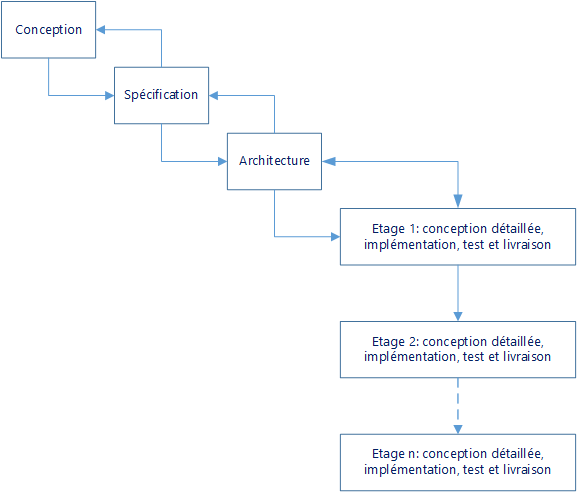
\includegraphics[width=100mm]{SDLC.png}
\caption{Cycle de vie de développement - Stage Delivery}
\end{figure}

\subsection{\Large Environnement de développement}
\vspace{0.2 cm}
\subsubsection{\large Développement}
Le développement sera réalisé en .NET (C\#) en utilisant \textbf{Visual Studio 2013 Ultimate} avec \textbf{Blend 4.0} pour améliorer les interfaces graphiques. Grâce à cette IDE, il est possible d'effectuer en même temps:
\begin{enumerate}
\item Architecture en UML
\item Implémentation des business logic
\item Implémentation de l'interface graphique
\item Tests unitaire et intégration
\item Test des performances
\end{enumerate}
Les langages principales utilisés sont \textbf{C\#5.0} et \textbf{XAML}.

\clearpage
\subsubsection{\large Contrôle de versions}

\textbf{Github} est utilisé pour gérer les versions de sources.Le mode de développement en adaptant la gestion des version de Git est le suivant: 
\begin{figure}[h!]
\centering
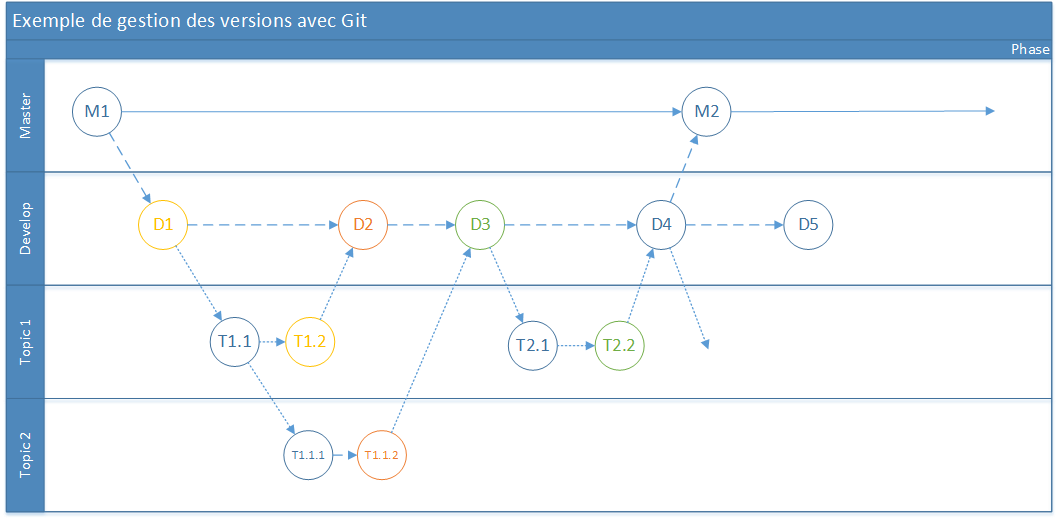
\includegraphics[width=150mm]{GIT.png}
\caption{Mode de travail en Git}
\end{figure}
\ \\\\Le branche \textbf{master} est maintenu pour les codes stables.
Les branches  \textbf{develop} est utilisés pour le développement (peut être instable partialement).
Les branches  \textbf{topic} est utilisés pour le développement des nouveaux fonctionnements.
\vspace{0.2 cm}
\subsubsection{\large Simulation, test et déploiement}
Le test générale de l'application sera faite avec l'\textbf{émulateur Windows Phone} d'IDE ou un mobile \textbf{Lumia 1020}.L'application finale sera publiée sur le Windows Phone Store. 
\\\\  
Car notre application fonctionne pendant tout le voyage, il faut créer un environnement assez complet pour pourvoir simuler toutes les possibilités. Une description complète de simulateur est mentionnée dans la section "Tests et simulation".


\newpage
\subsection{\Large Spécification fonctionnelle}

Après l'analyse du marché et du besoin, nous fixons une liste de spécification suivante. Cette liste n'est pas trop détaille car nous allons l'adapter et la spécifier pendant chaque étage de développement (Stage Delivery).

\begin{figure}[h!]
\centering
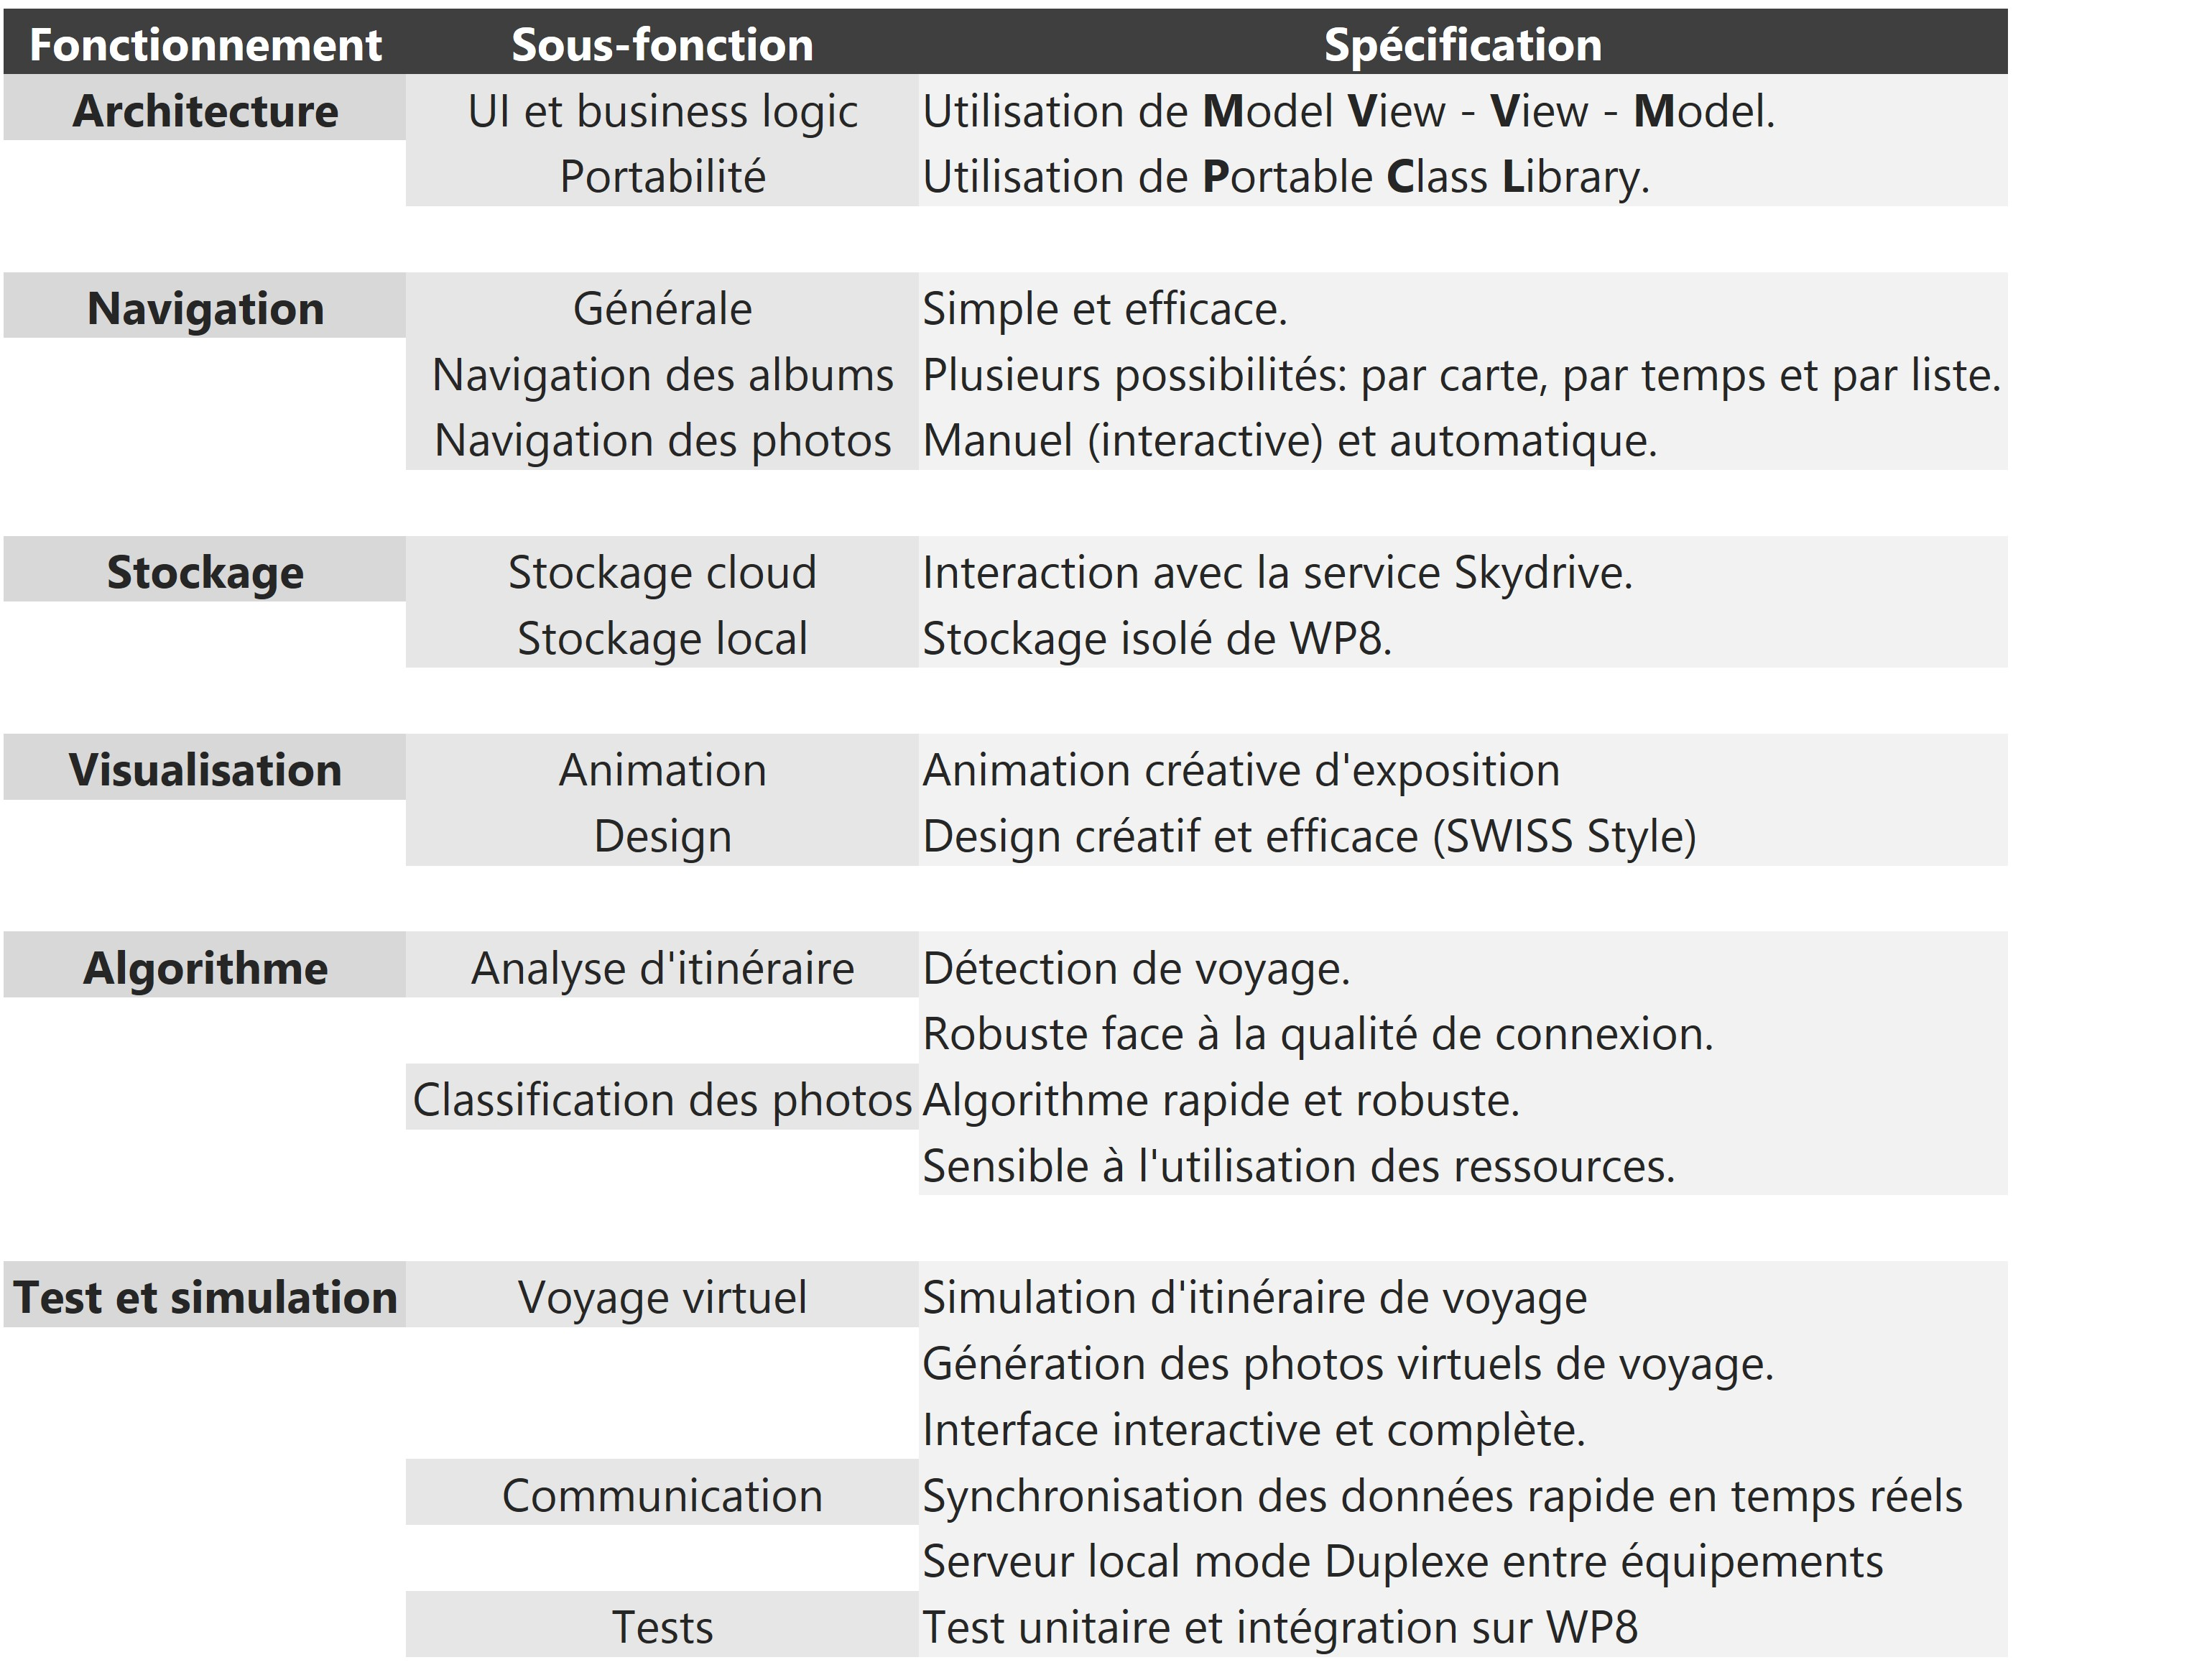
\includegraphics[width=180mm]{SPEC.jpg}
\caption{Spécification générale}
\end{figure}

\vspace{0.2 cm}
\subsection{\Large Livrables}

A la fin du projet, les livrables attendues devant être produits par l'équipe:
\begin{itemize}
\item Bibliothèque portable concernant des business logic (API PCL)
\item Application Windows Phone 8 concernant l'interface UI et le système d'informatique (XAP).
\item Simulateur de voyage (Windows Form)
\item Documentation SandCastle (HTML)
\end{itemize}


%----------------------------------------------------------------------------------------
% SECTION 3
%----------------------------------------------------------------------------------------
\newpage
\section{\LARGE ARCHITECTURE}

\vspace{0.2 cm}
\subsection{\Large L'architecture globale}

Le système global consiste en 4 parties: \textbf{application principale}, \textbf{application des test}, l'\textbf{agent du fond} et le \textbf{simulateur}. Leur relation est donnée par le schéma ci-dessous:
\begin{figure}[h!]
\centering
\includegraphics[width=150mm]{ARCHI2.pdf}
\caption{L'architecture générale du système}
\end{figure}

\begin{itemize}
\item Application principale: visualisation des albums.
\item Application des test: pilotage et communication avec le simulateur.
\item Agent du fond:  exécution de l'algorithme.
\item Simulateur: simulation de voyage et tests de fonctionnement.
\end{itemize}

\vspace{0.2 cm}
\subsubsection{\large Architecture sur Windows Phone 8}
L'application principale, l'application des tests ainsi que l'agent du fond sont réalisées dans l'environnement Windows Phone 8. Pour les deux applications, l'\textbf{architecture MVVM + PCL} est utilisée pour une meilleure portabilité et séparation du design et codage. Nous montrons en détail cette architecture dans les sous-sections suivantes.

\vspace{0.2 cm}
\subsubsection{\large Architecture de simulateur}
Le simulateur consiste en deux parties: \textbf{interface graphique} et \textbf{service de simulation}. Nous l'aborderons en détail dans la section "Simulateur".

\vspace{0.2 cm}
\subsubsection{\large Architecture de communication}
Il existe deux types de communication dans le système:  \textbf{REST} pour la partie synchronisation en Cloud et \textbf{WCF} pour l'échange des données avec le simulateur.
\\\\
Grâce à l'API de SkyDrive, \textbf{LiveSDK}, nous pouvons facilement effectuer les enquêtes REST au service SkyDrive. l'authentification est gérée par l'API pour rassurer la sécurité de compte. Une fois authentifiée, application peut effectuer les échanges avec la service Cloud SkyDrive en fond.

\vspace{0.2 cm}
\subsection{\Large L'architecture MVVM + PCL}

\vspace{0.2 cm}
\subsubsection{\large Model View ViewModel}
\textbf{Model View ViewModel} est une dérivé de \textbf{Model View Controller} pour générer la partie interface et la partie logique. Comme MVC, MVVM offre un couplage tellement faible qu'une modification de la interface graphique n'aura aucune impacte sur la partie logique et vice versa. Autrement dire, le Design et le Développement sont complètement isolés. 

\begin{figure}[h!]
\centering
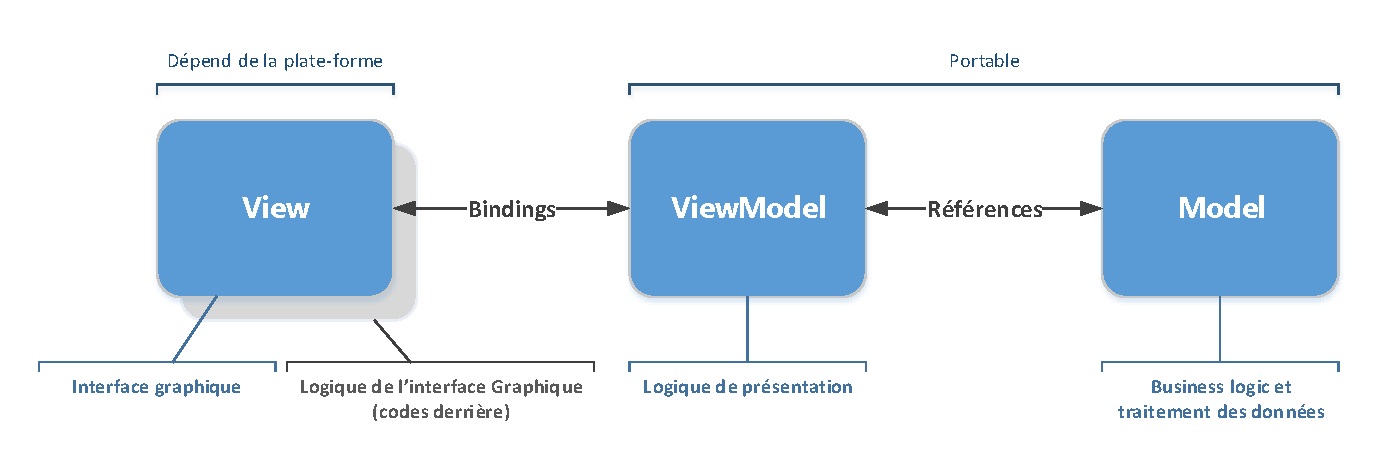
\includegraphics[width=150mm]{MVVM.pdf}
\caption{Architecture MVVM}
\end{figure}
\ \\Cependant MVVM profite beaucoup du framework .NET. Inspiré de la conception \textbf{Binding} et \textbf{Event} de .NET, MVVM donne une architecture plus sensible au couplage des ressource interface graphique et les données cachées derrières. 

\vspace{0.2 cm}
\subsubsection{\large Portable Class Library}
Le \textbf{Portable Class Library} est une API .NET sert à créer des applications portables. En utilisant le projet type PCL dans Visual Studio, une sous-partie portable des APIs .NET sont référencés. Elles sont portables en plusieurs plate-forme comme Windows Phone, Windows 8 voire Andriod, Linux et IOS. En effet, référencés par un autre projet de type spécifique, un compilateur va transformer les codes PCL en code spécifique du projet. 

\vspace{0.2 cm}
\subsection{\Large Inversion de Contrôle (IoC)}
Avec les deux architectures mentionnées précédentes, nous arrivons à créer un système structuré et portable. En revanche, il reste de faire la connexion entre les environnements différents (PCL et les plate-forme spécifique). 
\\\\
L’\textbf{inversion de contrôle (IoC)} est un patron d'architecture commun à tous les frameworks. Il fonctionne selon le principe que le flot d'exécution d'un logiciel n'est plus sous le contrôle direct de l'application elle-même mais du framework ou de la couche logicielle sous-jacente. 
\\
\begin{figure}[h!]
\centering
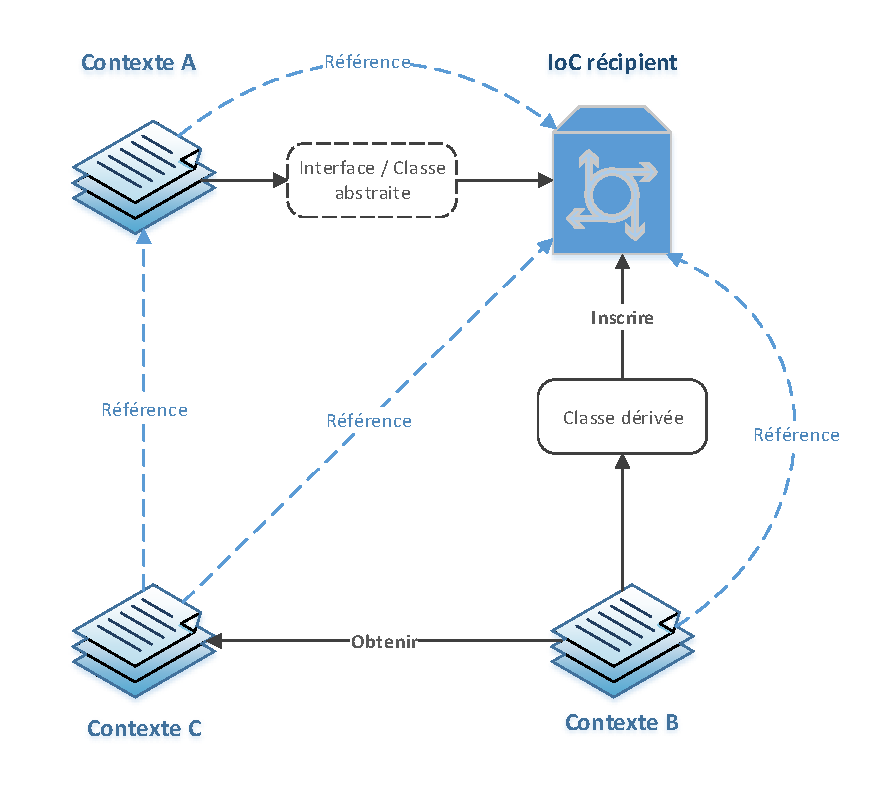
\includegraphics[width=120mm]{IOC.pdf}
\caption{Principe de l'IoC}
\end{figure}
\ \\\\
Prenons un example suivant, le programme A a déclaré une interface qui est référencée dans programme B. Pourtant la réalisation est effectuée dans le programme B. Or le programme C n'intéresse pas comment est réalisée l'interface. Par l'inscription (injection du programme B au récipient IoC), l'IoC conserve une instance de classe concrète. En utilisant le \textbf{Service Locateur}, le programme C peut facilement retirer l'interface sans connaître l'instance réelle. Comme ça, la contexte B et C sont isolées.

\newpage
\subsection{\Large L'architecture MVVM + PCL}

Nous allons implémenter le logique générale en PCL. Les implémentations concrètes spécifiques au plate-forme vont être injectées à l'aide du récipient IoC. 
\\\\
Pour ce projet, seulement les parties PCL et WP8 seront réalisées. Pourtant, l'extension à Windows Store Application est assez simple grâce à l'architecture PCL + MVVM. Il faut juste implémenter les interfaces selon les contraintes spécifique du plate-forme WP8 ainsi que les composants graphiques.
\\\\
Nous modélisons l'architecture générale de l'application à l'aide du diagramme des couches dans Visual Studio.

\begin{figure}[h!]
\centering
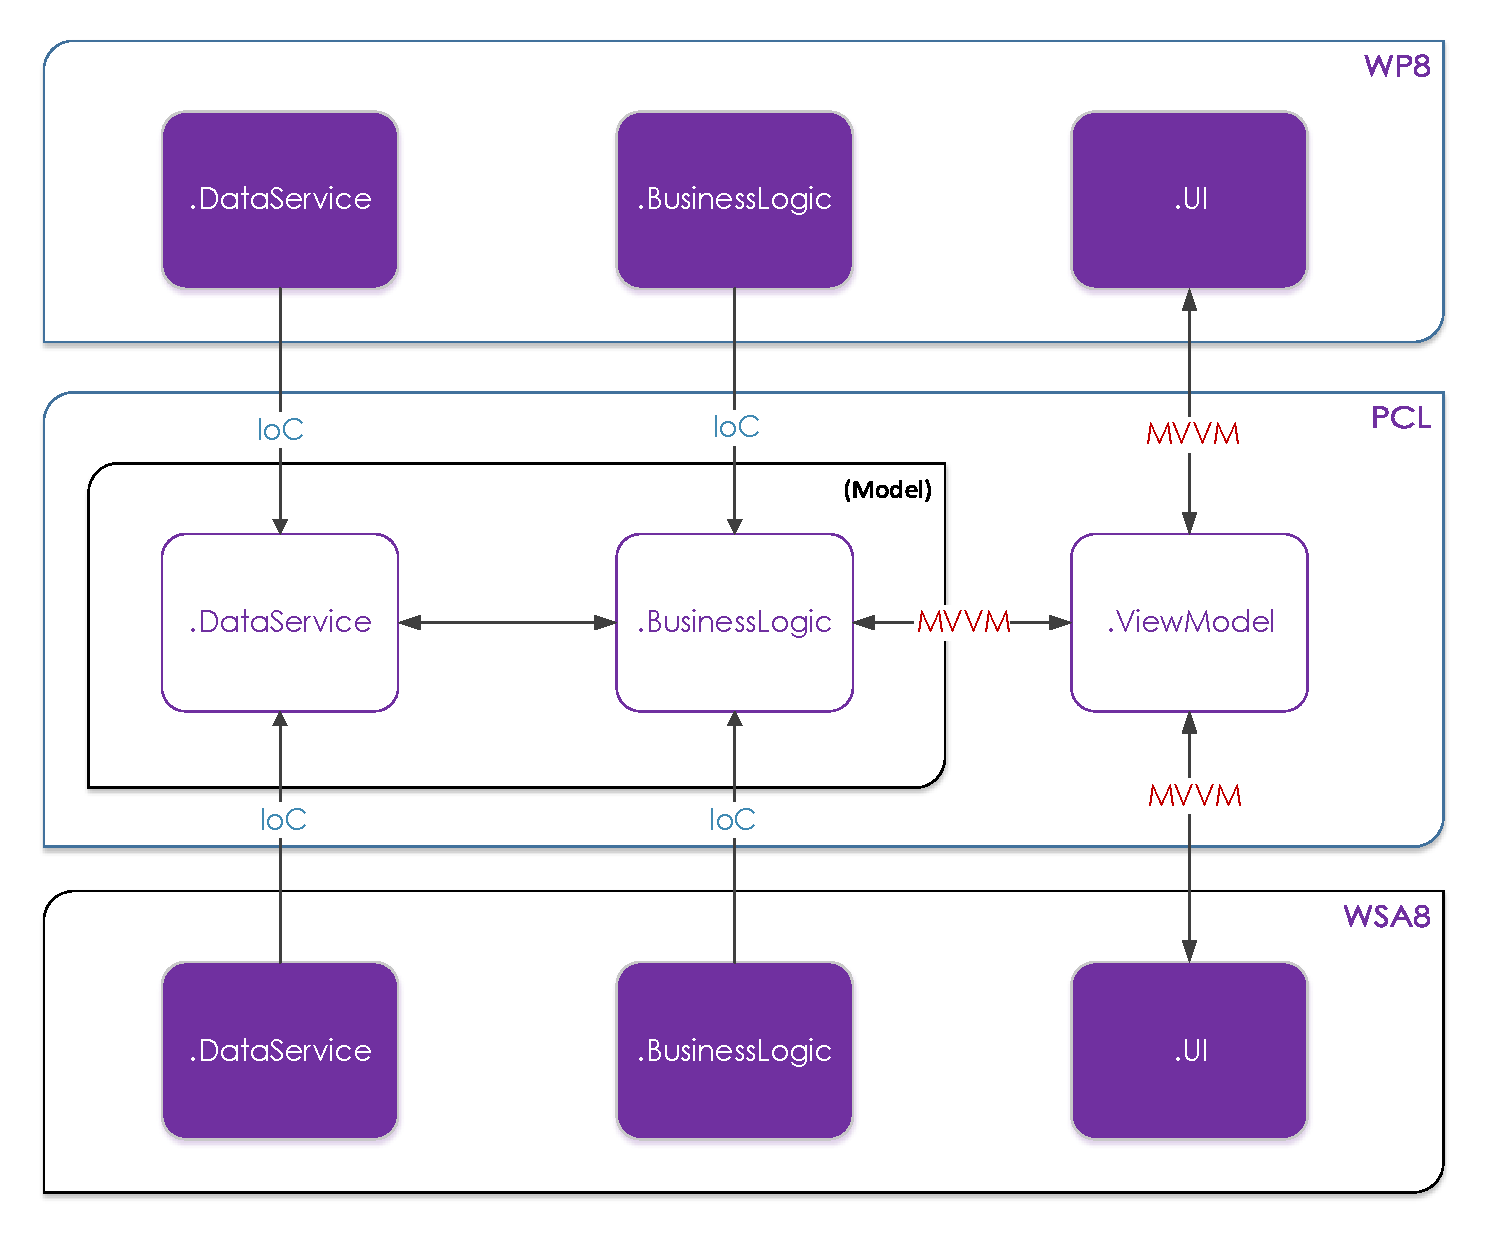
\includegraphics[width=150mm]{ARCHI.pdf}
\caption{L'architecture générale de l'application}
\end{figure}



%----------------------------------------------------------------------------------------
% SECTION 4
%----------------------------------------------------------------------------------------
\clearpage
\section{\LARGE ALGORITHME }

\vspace{0.2 cm}
\subsection{\Large Description générale}

L’algorithme principal de l’application est développé en architecture PCL. Afin de bien structurer nos programmes et afin que l’implémentation spécifique à la plate-forme WP8 ou l’extension d’application à Windows Store 8 seront facilement réalisable, nous rangeons des différents comportements d’objet à des différent classes ces qui sont bien abstraits.  Les étapes du fonctionnement et les différent tâches des classes ou interfaces sont expliqués comme le suivant :
\\\\
Le processeur arrière-plan (\textbf{BackgroundProcessor}) joue un rôle le plus important dans le processus d’exécution car il contrôle tous les comportements entre les autres classes(ou interfaces) et lui-même. 
\\\\
Le service web ({\bf IWebService}) peut obtenir des informations de l’emplacement de l’utilisateur et les transmet à Le processeur.
Il contient aussi des méthodes pouvant obtenir des informations de GPS pointe par {\bf Bing Maps REST Service}.
\\\\
{\bf DataManager} est une classe dont la tâche consiste à sérialiser des données locales, plus les enregistrer en nuage (OneDrive pour Windows)  et vice versa.  D’ailleurs, elle contient des méthodes qui peuvent être appelés pour chargement et déchargement des données entre  le processeur et lui-même.
\\\\
Après la réception des données actuels de l’utilisateur et des anciens données provenant de base de données, le processeur va déterminer à quelle état il est se situé. Si cette fois, le processeur est dans l’état {\bf PhotoHandlerState}, il effectuera des opérations suivantes pour traiter les informations des photos.  (Le fonctionnement en machine d’état est expliqué par la suite)
\\\\
{\bf IPhotoManager} se charge de tester l’existence des nouveaux photos qui sont pas encore traités, et si oui, il procède au traitement ces nouveaux photos. Nous utilisons une délégation ici afin de séparer la logique d’traitement de la méthode appelé.  De cette façon, {\bf IPhotoManager} peut réaliser sa tâche sans connaître de précisément de autres objets et sans accéder des ressources supplémentaires.
\\\\
Une fois que le processeur trouve du nouveau photo, il appelle la méthode d’{\bf IExifExtractor} pour tirer les données intéressants de GPS et les repasser à {\bf IWebService} pour obtenir finalement des informations d’emplacement.
\\\\
Attention, toutes les opérations ci-dessous ne sont pas sûrement terminées dans une fois d’exécution. Heureusement, les opérations qui ne sont pas terminées sont continuées à être traitées à la prochaine fois d’exécution. En effet, après avoir testé l’efficacité d’exécution, le résultat prouve que notre application se déroule sans problème.


\begin{figure}[h!]
\centering
\includegraphics[width=150mm]{SequenceDiagram.pdf}
\caption{Diagramme UML du fonctionnement du programme principal en architecture PCL}
\end{figure}
\newpage

\vspace{0.2 cm}
\subsection{\Large Contexte de fonctionnement}

Nous avons déjà vu le déroulement principal du programme, mais toutes les tâches ci-dessous doivent être exécutées sous une condition très importante. Windows Phone propose un système différent de gestion du multitâches. Ce n’est pas du multitâches à proprement parler, mais la possibilité de faire des choses de manière périodique en tâche de fond lorsque l’application est désactivée. Il s’agit des {\bf{Background Agent}}, qui sont de tâches qui s’exécutent en arrière-plan. Les tâches que nous utilisons pour notre application sont les tâches périodiques. Une tâche périodique doit être exécutée assez rapidement et doit faire quelque chose de simple, comme mettre à jour de nouvelles photos et tirer des informations de GPS dans notre cas. Ces tâches sont exécutées toutes les 30 minutes, sont limitées en nombre par téléphone (cela dépend de la configuration du téléphone) et ne dépassent pas 25 secondes d’exécution.
\\\\
Nous utilisons ce système pour notre application non seulement pour la besoin de fonctionnement périodique, mais aussi pour la simplicité des tâches étant souhaitées à effectuer. Pendant l’implémentation, nous avons essayé d’utiliser des tâches asynchrones mais il y avait pleine de bugs et quand nous les modifiions en manière synchrone, nous avons trouvé ceux-ci  sont plus faisable et assez efficace.


\vspace{0.2 cm}
\subsection{\Large Fonctionnement en machine d'état}

\newpage
\begin{figure}[h!]
\centering
\includegraphics[width=100mm]{StateMachine.pdf}
\caption{Cycle de la machine d'état}
\end{figure}
\ \\
Etant donné qu’il existe plusieurs états possibles pour l’utilisateur et pour des photos, par exemple,  l’emplacement de l’utilisateur est toujours variable et des photos sont faites arbitrairement pendant du voyage, c’est mieux que partager des tâches d’opération en partie différentes selon des états différentes  afin que chaque états s’occupe des tâches nécessaires sans des opérations superflues.
\\\\
Nous modélisons quatre états pour une cycle du fonctionnement, soit le premier état : {\bf OriginalState }; le deuxième état : {\bf PioltState} ; le troisième état : {\bf PhotoHandleState} ; le quatrième état : {\bf AlbumGeneratorState} ; 
\\\\
Tout d’abord, le programme tourne toujours dans l’état {\bf OriginalState} si l’utilisateur ne sortit pas de sa ville originale. Dans cet état-là, il n’y a aucune opération.
\\\\
Une fois que utilisateur n’est plus à sa ville originale et il n’y a pas encore des nouveaux photos, on passer au état suivant-{\bf Pioltstate}. Pour cet état, il n’y a pas d’opération sauf que l’enregistrement des informations de GPS de l’utilisateur.
\\\\
Si maintenant quelques photos sont générées, l’état est mise à jour en même temps. On arrive à l’état {\bf PhotoHandlerState}, ce qui sert à traiter des informations des photos. On note des GPS points des nouveaux photos et plus obtient des informations de l’emplacement (pays, province, ville etc.) sur la base des GPS points. De même, on enregistre aussi des informations de GPS de l’utilisateur comme l’état précédent. Evidemment, l’état {\bf OriginalState} peut traverser directement à l’état {\bf PhotoHandlerState} sans passer l’état {\bf PioltState} en certains cas.
\\\\
Quand l’utilisateur retourne dans sa ville originale et toutes les photos sont bien traitées, on passe à l’état final- l’état {\bf AlbumGeneratorState}. Le but de cet état est l’organisation des albums des photos. On obtient un ensemble des noms des villes visités en parcourant toutes les photos existant et enlève des GPS points de l’utilisateur dont la ville n’a aucune photo. Lorsque ces tâches sont tous finis, on repasse à l’état original.

%----------------------------------------------------------------------------------------
% SECTION 5
%----------------------------------------------------------------------------------------
\newpage
\section{\LARGE APPLICATION }

\vspace{0.2 cm}
\subsection{\Large Description générale}

Comme nous avons mentionné dans la section précédente, l'application va fonctionner principalement en fond. Nous présentons ci-dessous la cycle de vie générale de l'application avec un \textbf{diagramme BPMN 2.0}.

\begin{figure}[h!]
\centering
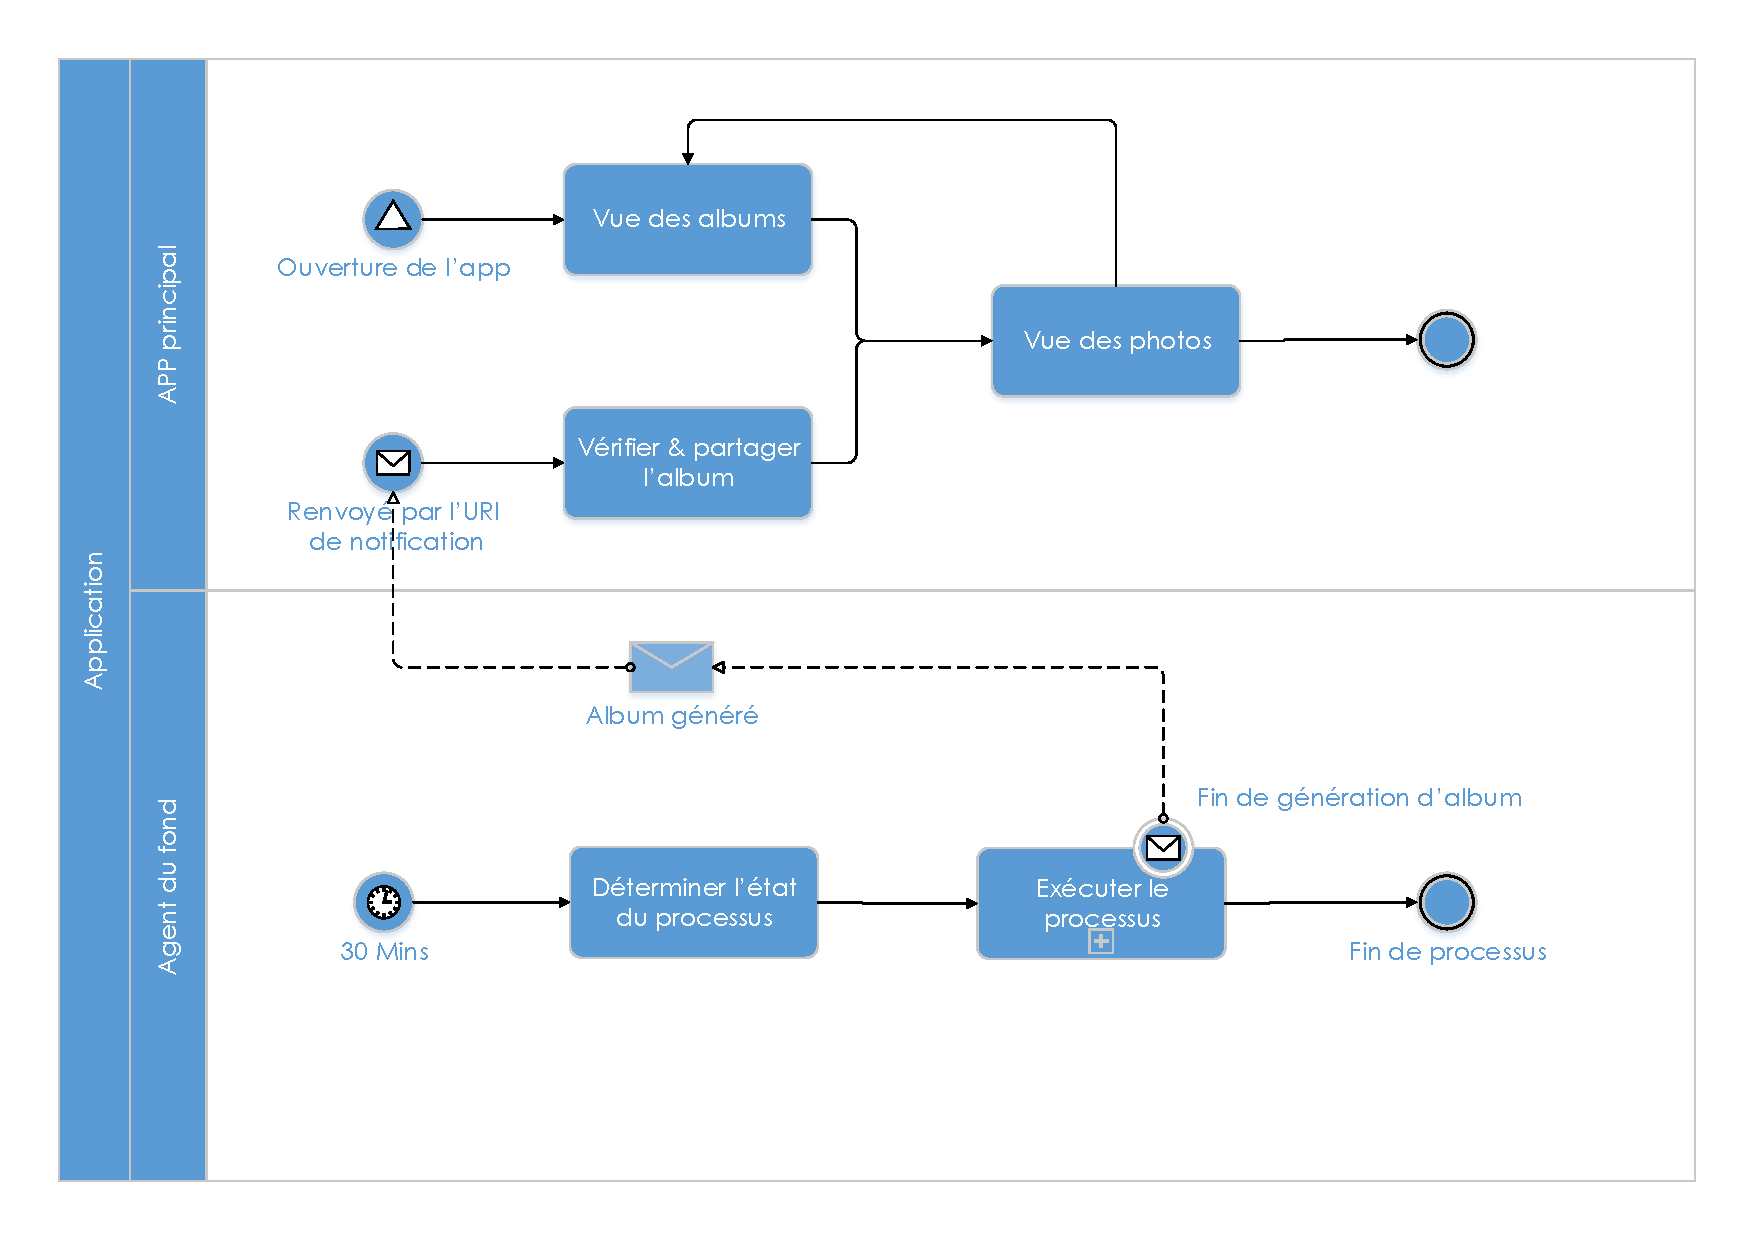
\includegraphics[width=160mm]{APP.pdf}
\caption{Cycle de vie générale de l'application}
\end{figure}

\ \\L'application se divise en deux parties séparées: \textbf{application principale} et l'\textbf{agent du fond}. Dans l'application principale, l'utilisateur peut visualiser les photos et albums pris pendant un voyage. En même temps, l'agent du fond travaille sans cesse pour détecter un voyage et générer les albums. 

\vspace{0.2 cm}
\subsection{\Large Navigation des photos}

Nous envisageons trois modes pour naviguer entre les photos: 

\begin{itemize}
\item la vue normal (navigation simple par les gestes simples)
\item la vue par la liste des photos
\item la vue par la carte
\end{itemize}

\begin{figure}[h!]
\centering
\begin{subfigure}{.3\textwidth}
  \centering
  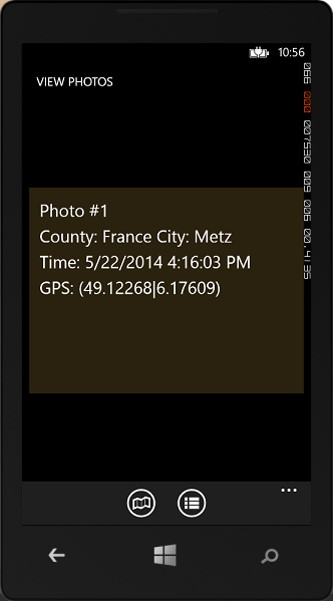
\includegraphics[width=.9\linewidth]{Phone1.jpg}
\end{subfigure}%
\begin{subfigure}{.3\textwidth}
  \centering
  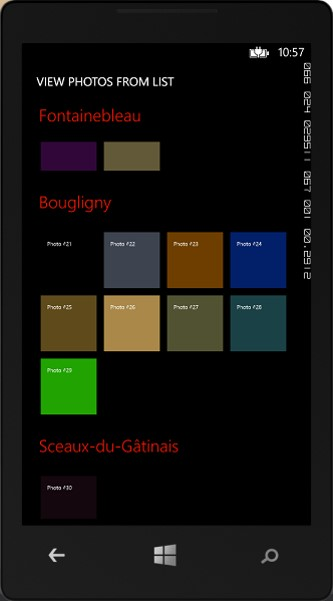
\includegraphics[width=.9\linewidth]{Phone2.jpg}
\end{subfigure}
\begin{subfigure}{.3\textwidth}
  \centering
  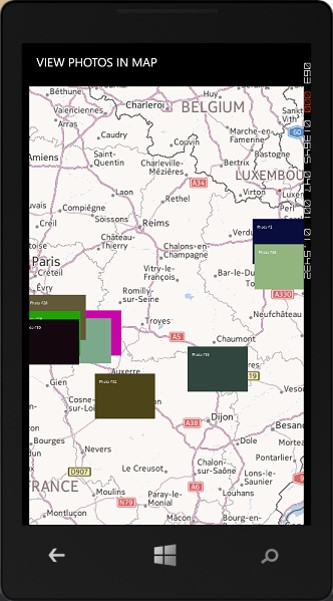
\includegraphics[width=.9\linewidth]{Phone3.jpg}
\end{subfigure}
  \caption{Navigation entre les photos}
\end{figure}

\vspace{0.2 cm}
\subsubsection{\large Vue normale}
Dans la vue normale, utilisateur peut naviguer en gauche et à droite les photos par la vue classique d'un album. Aussi, l'utilisateur peut zoomer et dézoomer sur un photo avec les gestes correspondantes.

\vspace{0.2 cm}
\subsubsection{\large Vue par liste}
Nous réalisons un vue par \textbf{"jump-list"} pour rendre plus facile la navigation non-linéaire des photos. L'utilisateur peut entrer dans cette vue en cliquant sur le bouton en bas du page. Les photos sont regroupé en fonction des position (ville et pays). Grâce au jump-list, utilisateur peut facilement naviguer au groupe désiré en cliquant sur l'entête des groupes puis choisir le groupe correspondante.  

\vspace{0.2 cm}
\subsubsection{\large Vue par carte}
Nous réalisons un vue par \textbf{carte} pour mieux présenter les photos selon leur position ainsi que l'itinéraire de voyage. Cette vue  est basée sur le contrôle  \textbf{carte} de Windows Phone 8. Les photos sont placés dans la carte en tant que les étiquettes relatives géographiques situées dans une couche séparée. Grâce à cette configuration, la détection des gestes différentes comme le déplacement de la carte et la sélection du photo peuvent être facilement réalisée.  Une animation de localisation est réalisée pour rendre plus dynamique la visualisation initiale des photos sur la carte.
\newpage
\subsection{\Large Visualisation}

Comme la visualisation joue un rôle très important dans l'application principale, nous réalisons plusieurs implémentations visuelles dans le prototype. Les éléments marqué avec un astérisque seront implémentés dans les versions futures.

\begin{figure}[h!]
\centering
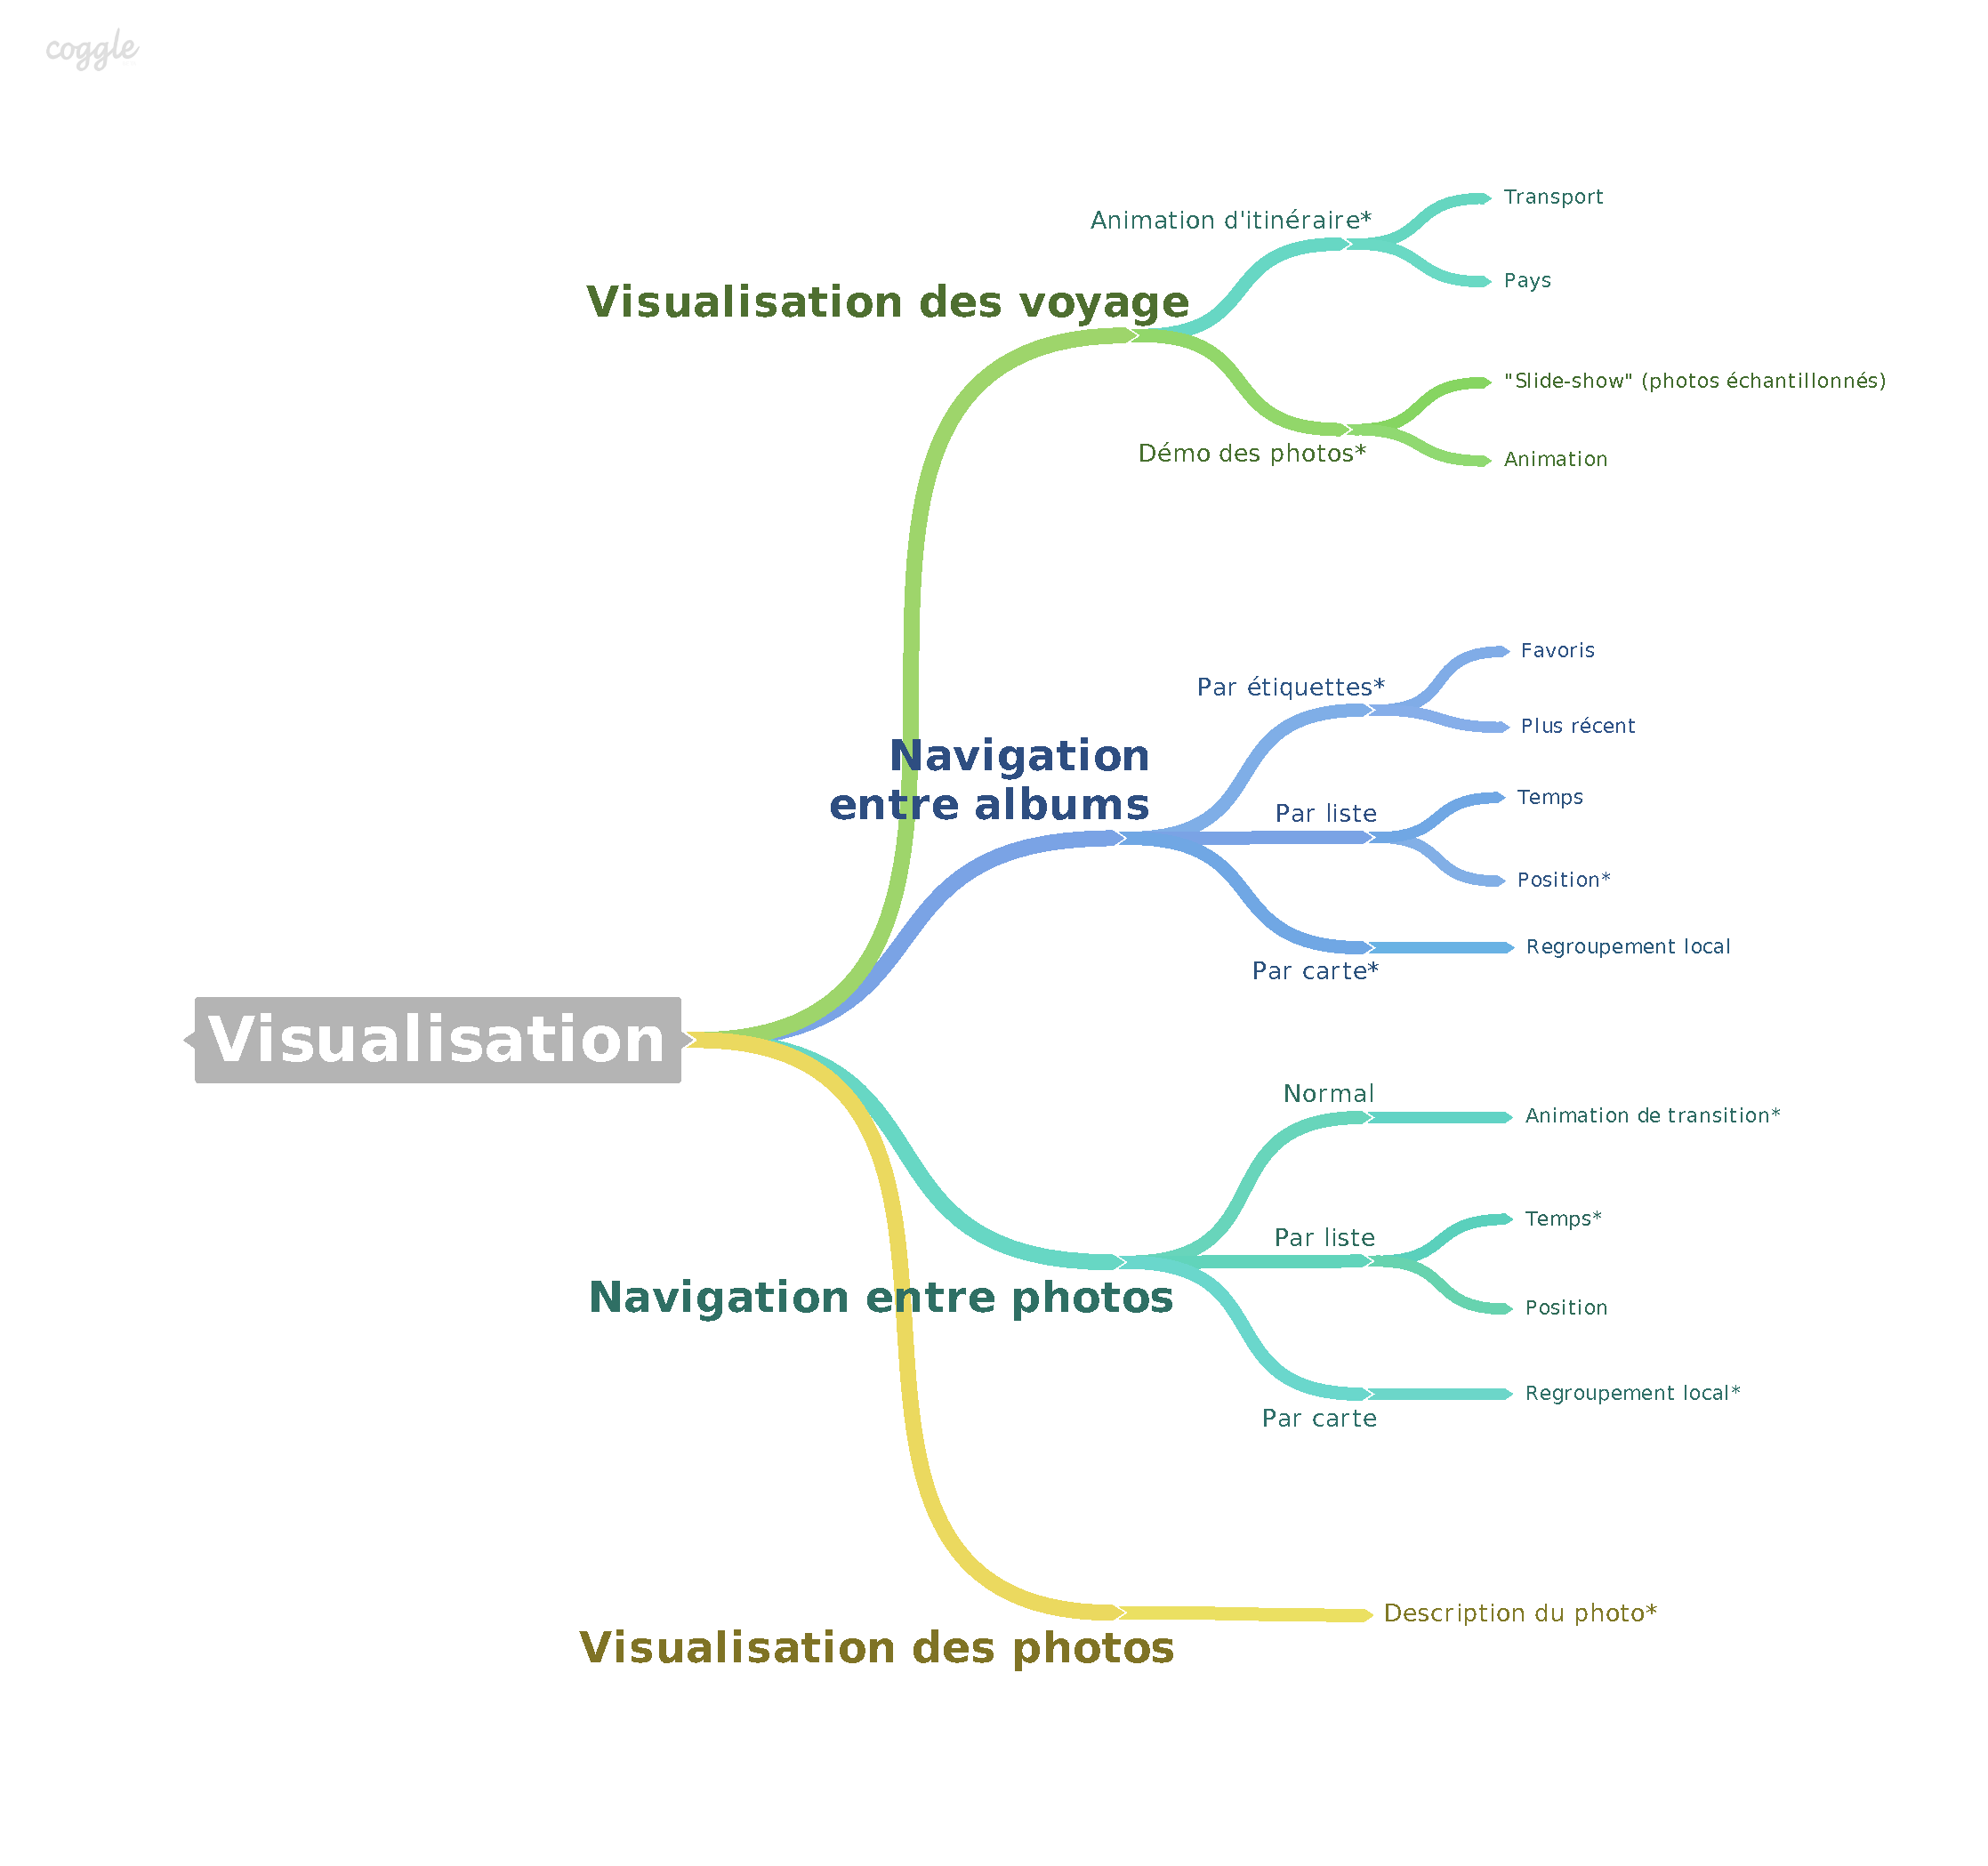
\includegraphics[width=160mm]{VISU.pdf}
\caption{Éléments de visualisation}
\end{figure}

%----------------------------------------------------------------------------------------
% SECTION 6
%----------------------------------------------------------------------------------------
\clearpage
\section{\LARGE SIMULATEUR }

\vspace{0.2 cm}
\subsection{\Large Description générale}
Le simulateur consiste en deux parties générales: interface d'utilisateur et une service établie localement. Il permet la planification d'itinéraire de voyage, la génération des photos virtuels, la simulation en temps réel, etc.
\\\\
La technologie utilisée pour communiquer entre le simulateur et l'application mobile est \textbf{Windows Communication Foundation (WCF)}. Elle est une framework introduite en C\# 3.0 pour unifier les méthodes différentes de communication en Windows. Les détailles sont données dans les sous-sections suivantes. 
\begin{figure}[h!]
\centering
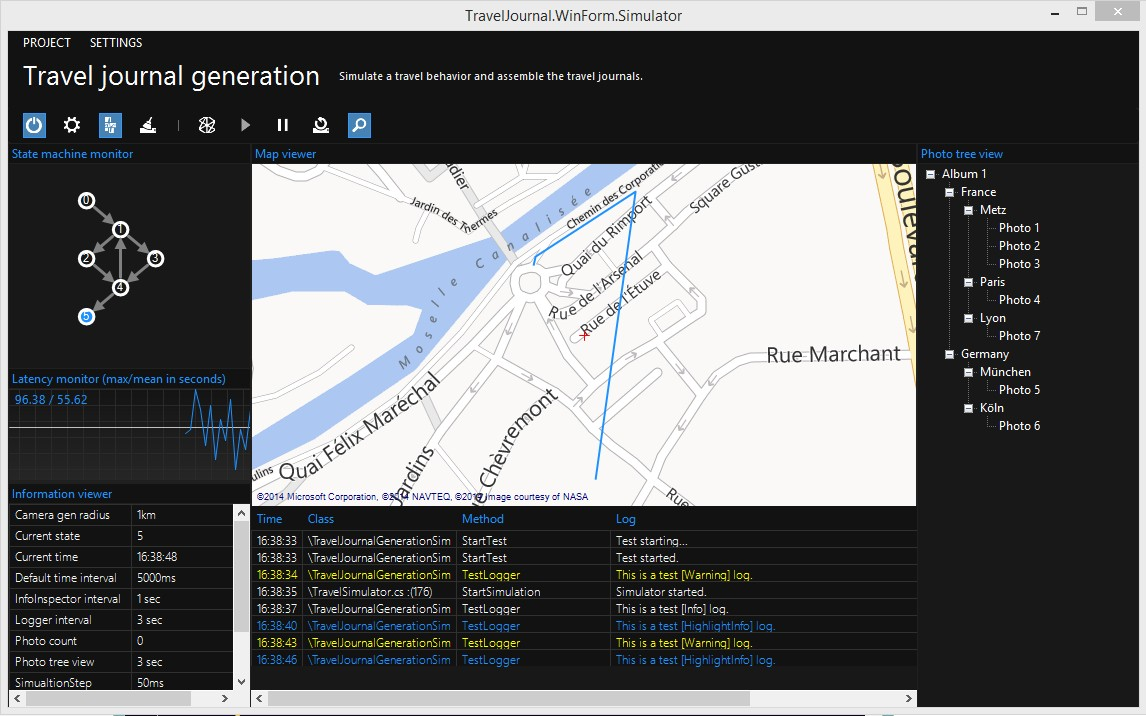
\includegraphics[width=160mm]{SIMU.jpg}
\caption{Interface de simulateur}
\end{figure}

\vspace{0.2 cm}
\subsection{\Large Interface graphique}
La partie interface du simulateur consiste en plusieurs modules:
\begin{itemize}
\item console de contrôle pour gérer la simulation et la configuration
\item moniteur de la \textbf{carte} pour visualiser le voyage
\item moniteur d'\textbf{état du programme} pour visualiser l'état du processeur (c.f. section 5.3) 
\item moniteur d'\textbf{information} pour visualiser les données intermédiaires
\item moniteur des \textbf{albums} générés
\item moniteur de \textbf{connexion entre serveur (Simulateur) et client (Windows phone)}
\item moniteur des \textbf{logs} pour le debug
\end{itemize}

\vspace{0.2 cm}
\subsubsection{\large Contexte de fonctionnement}
Chaque moniteur travaille dans son propre \textbf{Thread}, c'est-à-dire tout est doublement amorti. Cela conduit à donner une animation plus lisse. Mais cette configuration demande une ressource allouée plus importante. 

\vspace{0.2 cm}
\subsubsection{\large Transmission des données}
Pour la transmission des données entre modules, nous utilisons la \textbf{Sérialisation}. Cela permet aussi de vérifier la donnée en tout moment par la visualisation d'XML. Le mécanisme utilisé est la sérialisation WCF qui s'appelle \textbf{Data Contract Serialization}.
\\\\Héritées de la classe ConfigDataBase, toutes les classes de données utilisent le \textbf{patron d'Observateur}. Une fois une donnée est modifiée, tous modules la observant seront mis à jour. La réalisation profite de les notions d'\textbf{événement} et \textbf{propriété} de .NET: deux événements ( \textbf{OnDataChanging} et  \textbf{DataChanged}) seront invoqués lors la donnée est modifiée par le Setter.
\\\\De plus, la classe ConfigDataBase expose une méthode abstraite Display() qui permet au moniteur d'information d'inspecter ces données. 

\vspace{0.2 cm}
\subsubsection{\large Contrôle de la carte}
Nous utilisons la contrôle \textbf{Great Map Control} pour visualiser et inter-opérer avec la carte. Une documentation complète est donnée sur son site officiel.  

\vspace{0.2 cm}
\subsubsection{\large Révocation}
Le \textbf{patron de Memento} est utilisé pour rendre possible l'annulation de toute opération effectuée. Ceci est important pendant la construction d'itinéraire de voyage.

\vspace{0.2 cm}
\subsection{\Large Simulateur}
La simulateur est responsable de deux missions: la génération des données et la simulation en temps réel. 

\vspace{0.2 cm}
\subsubsection{\large Données de voyage}
Les données de voyage initiale sont présentées par les "ancres" de voyage. Il s'agit des \textbf{GPS} avec le \textbf{nombre de photos} seront pris dans le proche (N). Le testeur va les créer par un designer de la carte. Une fois enregistrées, ces données seront interprétées par un \textbf{compilateur} de simulation. Un \textbf{générateur aléatoire gaussienne} va générer N nouveaux GPS avec 1 photos pour chaque GPS initiale. Ensuite, ces données compilées seront traitées par le simulateur pour simuler un voyage. 
\\
\begin{figure}[h!]
\centering
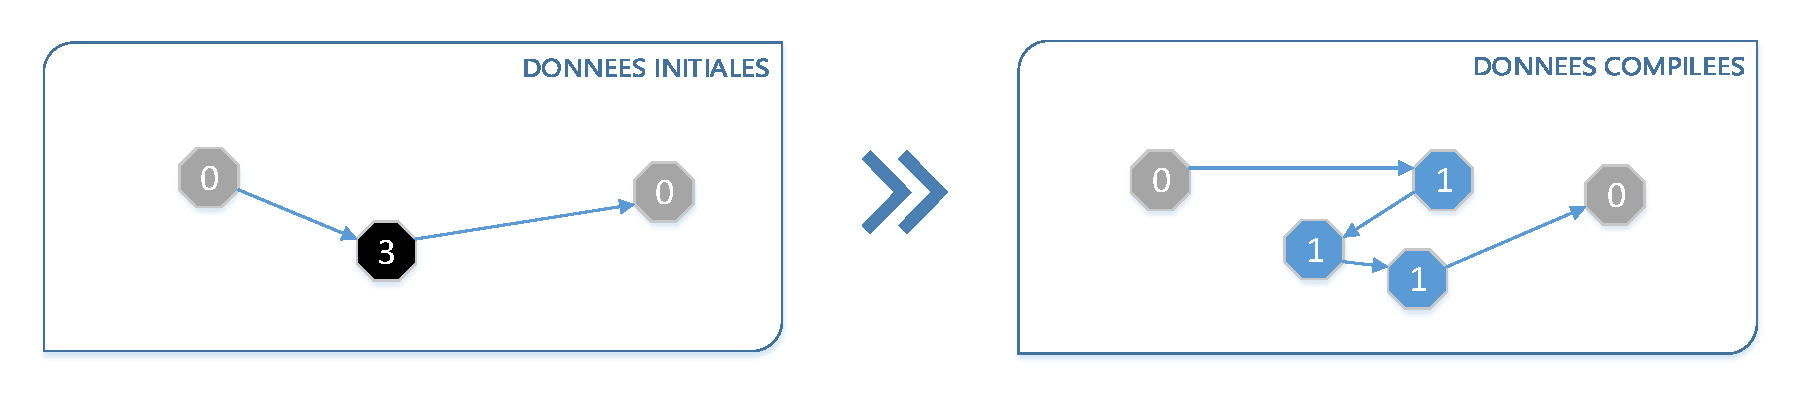
\includegraphics[width=150mm]{TRAVELDATA.pdf}
\caption{Génération des données de voyage}
\end{figure}
\\\\ Cette configuration modélise effectivement la prise des photos comme car elle dépende normalement de la location géographique.
\\\\ La durée de voyage entre deux "ancres" sont la même. C'est-à-dire pour modifier la vitesse, il suffit de modifier la distance entre des "ancres". Pour une distance identique, plus il y a des "ancres", moins elle est la vitesse.
\\\\ De plus, la ville d'habitation est indiquée lors la création de voyage.
\vspace{0.2 cm}
\subsubsection{\large Simulation}
La simulation de voyage est conduite par un \textbf{Timer}. Une fois les données de voyage sont générées et compilées, elles sont chargées dans le simulateur. Un \textbf{curseur (GPS)} va parcourir toute la route et retourner à la fin à l'origine. Tous les photos "prises dans le voyage"  (un photo est prise quand le GPS avec ce photo est parcouru par le curseur) sont enregistrés dans une liste pour donner ultérieurement à l'application mobile via les services WCF.

\vspace{0.2 cm}
\subsection{\Large Services WCF}
Les services \textbf{Windows Communication Foundation (WCF)} jouent un rôle très important dans la simulation. Elles permit la communication entre le simulateur et le mobile. 
\\\\
WCF est un modèle de programmation introduite en C\# 3.0 pour unifier les méthodes différentes de communication en Windows. \textbf{Inter-opérabilité} est la caractéristique fondamentale de WCF. Elle est composée de plusieurs éléments de Web Service, Remoting, MSMQ et COM+. Dans un mot, elle donne un plate-forme commune pour toutes les moyennes de communication dans le monde .NET. 
\\\\
Particulièrement, la programmation est simple avec WCF. L'utilisation des attributs facilite beaucoup l'implémentation des services du serveur. Un service WCF est composé de trois parties: 
\begin{itemize}
\item Une classe service
\item Un environnement hôte
\item Un ou plusieurs points finaux
\end{itemize}

\vspace{0.2 cm}
\subsubsection{\large Classe service}
La classe service n'est rien d'autre qu'une interface/classe décorée de quelques attributs WCF. 
\begin{lstlisting}[label=Example d'une classe service WCF,caption=Example d'une classe service WCF]
	    
    [ServiceContract]
    public interface ISimulationServices
    {
        #region Connection services
       
        [OperationContract]
        bool Connect(string deviceName);
      
        [OperationContract]
        bool Disconnect(string deviceName); 
      
        #endregion
    }
    
    [ServiceBehavior(InstanceContextMode = InstanceContextMode.Single)]
    public class SimulationServices : ISimulationServices
    {
          #region Connection services

        public bool Connect(string deviceName)
        {
        	...
        }
        public bool Disconnect(string deviceName)
        {
            ...
        } 

        #endregion
    }
\end{lstlisting}
\ \\
Les attributs utilisés permet à WCF de repérer les classes services lors la compilation.
\\\\
A l'exécution, WCF va gérer la transmission des données via la \textbf{Sérialisation WCF}, c'est-à-dire tous les augments et la valeur retournée vont être sérialisés et désérialisés pour être utilisés à distance. 

\vspace{0.2 cm}
\subsubsection{\large Environnement hôte et points finaux}
Dans la contexte de notre simulateur, le service est ''hosté" localement dans le simulateur (Application Windows Forme). Nous avons choisi cette configuration car le service ne sert qu'à la simulation de l'application --- le simulateur sera forcément ouvert. Pour configurer le hôte, il suffit de modifier la fichier de configuration "app.config":
\begin{lstlisting}[label=Configuration de hôte WCF,caption=Configuration de hôte WCF]

<system.serviceModel>
        <behaviors>
            <serviceBehaviors>
                <behavior name="">
                    <serviceMetadata httpGetEnabled="true" httpsGetEnabled="true" />
                    <serviceDebug includeExceptionDetailInFaults="false" />
                </behavior>
            </serviceBehaviors>
        </behaviors>
        <services>
            <service name="TravelJournal.WinForm.Simulator.SimulationServices">
                <endpoint address="" binding="basicHttpBinding" contract="TravelJournal.WinForm.Simulator.ISimulationServices">
                    <identity>
                        <dns value="localhost" />
                    </identity>
                </endpoint>
                <endpoint address="mex" binding="mexHttpBinding" contract="IMetadataExchange" />
            </service>
        </services>
        <bindings />
        <client />
    </system.serviceModel>
\end{lstlisting}
\ \\Un point final est un portail pour la communication. Il est composé d'une \textbf{adresse}, un \textbf{binding} et un \textbf{contrat}.
\\\\L'adresse de service est locale selon l'adresse IP de l'ordinateur. Le binding est en fait le protocole utilisé pour communiquer avec le service WCF. Nous utilisons le \textbf{BasicHttpBinding} qui utilise HTTP comme le protocole de transmission et XML comme l'encodage de message. Il est non sécurisé et faible au niveau de inter-opérabilité, cependant il est facile d'implémenté et 
est suffisant pour la simulation. Le contrat est l'interface ISimulationServices déclarée dans le codes.

\vspace{0.2 cm}
\subsubsection{\large Environnement hôte et points finaux}
Comme le service est "hosté" dans le simulateur, il faut ouvrir le simulateur pour mettre à jours le service.  La mise à jours est occupée automatiquement par l'IDE. 
\begin{figure}[h!]
\centering
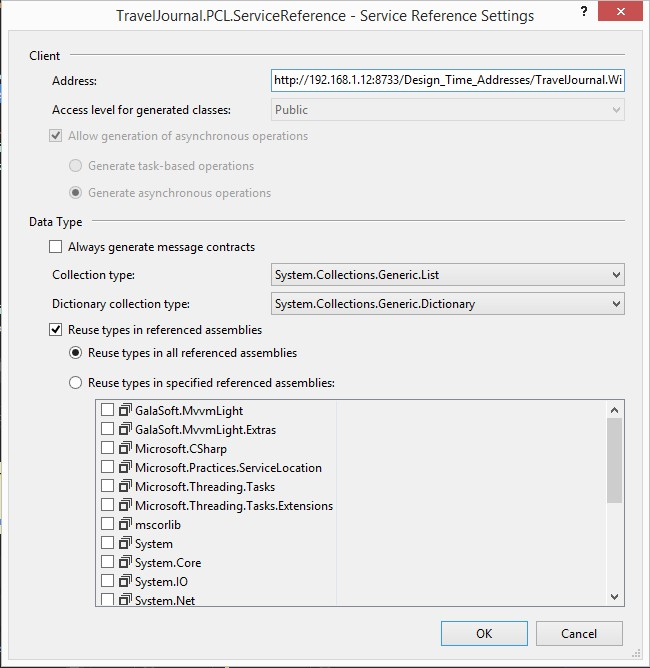
\includegraphics[width=80mm]{UPSERVICE.jpg}
\caption{La mise à jour automatique de service côté client}
\end{figure}

%----------------------------------------------------------------------------------------
% SECTION 7
%----------------------------------------------------------------------------------------
\vspace{2cm}
\section{\LARGE TESTS ET SIMULATIONS }
Pour travailler efficacement et agilement, nous faisons les test unitaires régulièrement dans l'implémentation de business logic. Ensuite, les test de transmission sont faits pour pouvoir lancer une simulation complète. A la fin, une simulation complete de voyage est effectuée. 

\vspace{0.2 cm}
\subsection{\Large Test unitaires}

Un test unitaire consiste en 3 parties: \textbf{arrangement}, \textbf{action} et \textbf{assertion}. Grâce à l'IDE, les tests sont automatisés et l'implémentation peut facilement basée en test (Test Driven Développement). Nous allons modifier l'implémentation jusqu'à la "passe" de tous les tests. Voici un exemple de test unitaire sur l'extraction des données EXIF de photo. 

\begin{lstlisting}[label=Exemple de test unitaire,caption=Exemple de test unitaire]

[TestClass()]
    public class ExifLibExtractorTests
    {
        [TestMethod()]
        public void ExtractGeoCoordinateTest()
        {
            // Arrange
            ExifLibExtractor extractor = new ExifLibExtractor();
            MediaSource mediaSource = MediaSource.GetAvailableMediaSources().First((source => source.MediaSourceType == MediaSourceType.LocalDevice));
            Picture samplePicture;
            using (MediaLibrary mediaLibrary = new MediaLibrary(mediaSource))
            {
                PictureAlbum cameraRollAlbum = mediaLibrary.RootPictureAlbum.Albums.First((album) => album.Name == "Camera Roll");
                samplePicture = cameraRollAlbum.Pictures.First();
            }
            Photo photo = new Photo()
            {
                Name = "WP_20131201_13_37_04_Pro.jpg"
            };
            // Act
            GpsPoint point = extractor.ExtractGeoCoordinate(photo);
            // Assert
            Assert.AreNotEqual(default(double),point.Latitude);
            Assert.AreNotEqual(default(double), point.Longitude);
            Assert.AreNotEqual(default(DateTime), point.Timestamp);
        }
    }

\end{lstlisting}
\newpage
\subsection{\Large Test de transmission }
 
Pour le test d'intégration, nous créons un client mobile pour lancer l'agent du fond. Le client dispose de 3 tests: \textbf{test de connectivité du service} et \textbf{test d'information de voyage}. 

\vspace{0.2 cm}
\subsubsection{\large Test de connectivité du service}
Ce test destine à tester la connectivité du serveur et client. Il est composé de deux tests: échange d'un paquet entre le simulateur et le client et un processus périodique de même opération. Dans ces tests, une liste des entières est utilisée.  
\begin{figure}[h!]
\centering
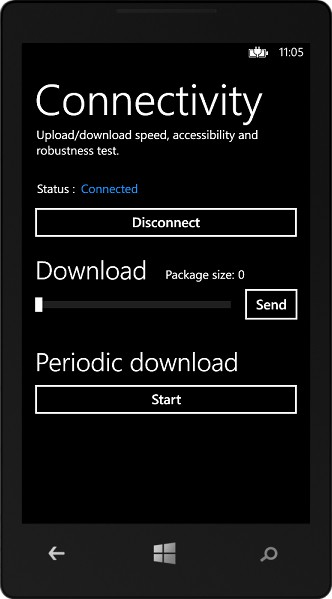
\includegraphics[width=50mm]{TESTCONNECT.jpg}
\caption{Test de connectivité}
\end{figure}
Testé avec la connexion locale (simulateur et émulateur WP ), la délai d'échange d'un paquet de \textbf{500000/1000000} éléments vaut \textbf{0.89/1.23 seconds}. Le dernière paquet utilisé est supérieur à la taille de donnée réelle de simulation. Donc la vitesse de communication est assurée, nous pouvons négliger la délai de transmission.

\newpage
\subsubsection{\large Test d'information de voyage}
Ce test destine à tester le téléchargement des photos générés par le simulateur. Après ce test, nous pouvons considérer que l'échange est bien définie alors la partie de transmission est assurée pour une simulation complète.

\begin{figure}[h!]
\centering
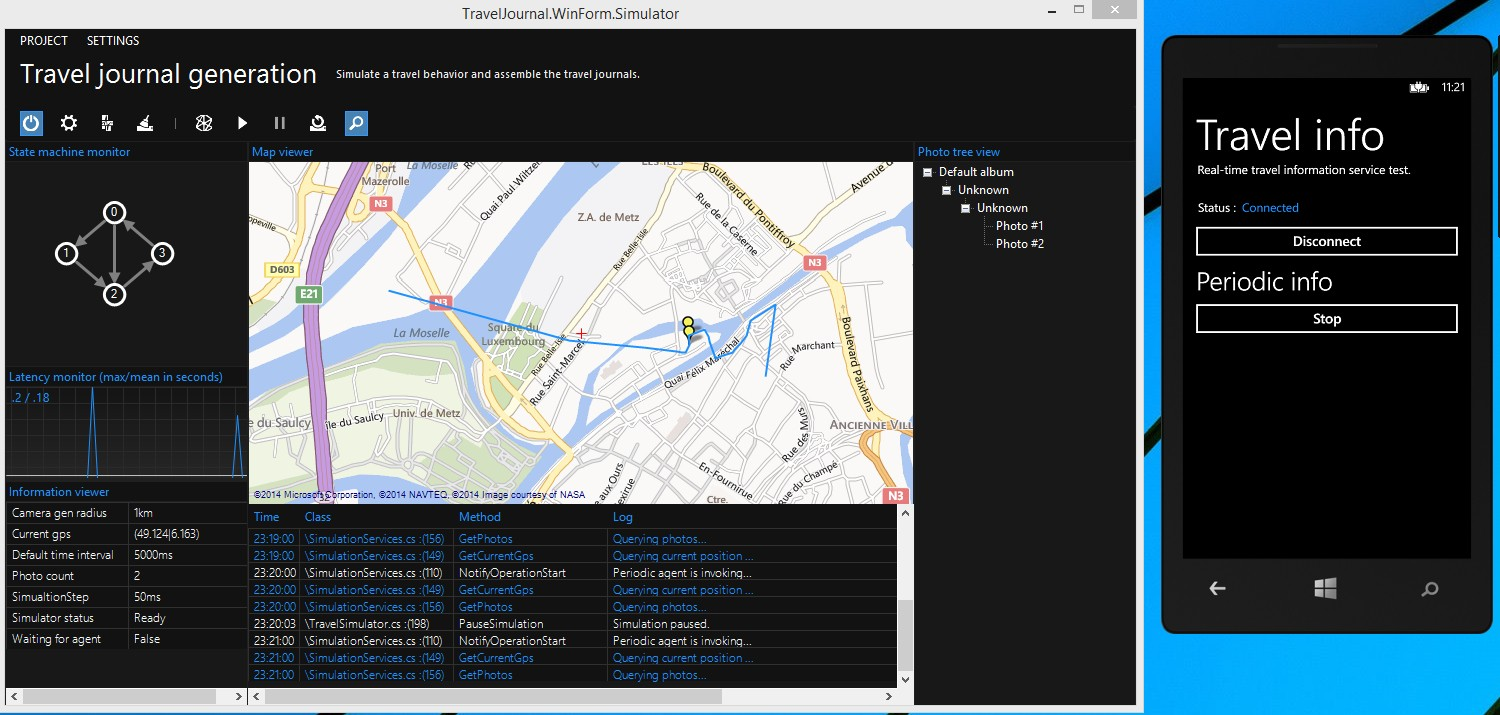
\includegraphics[width=150mm]{TESTINFO.jpg}
\caption{Test d'information de voyage}
\end{figure}

\vspace{0.2 cm}
\subsection{\Large Simulation}

La simulation complète est basée sur un voyage à partir de Metz avec 36 photos. Au début, le curseur est à Metz, alors le programme reste à l'état initial. 
\begin{figure}[h!]
\centering
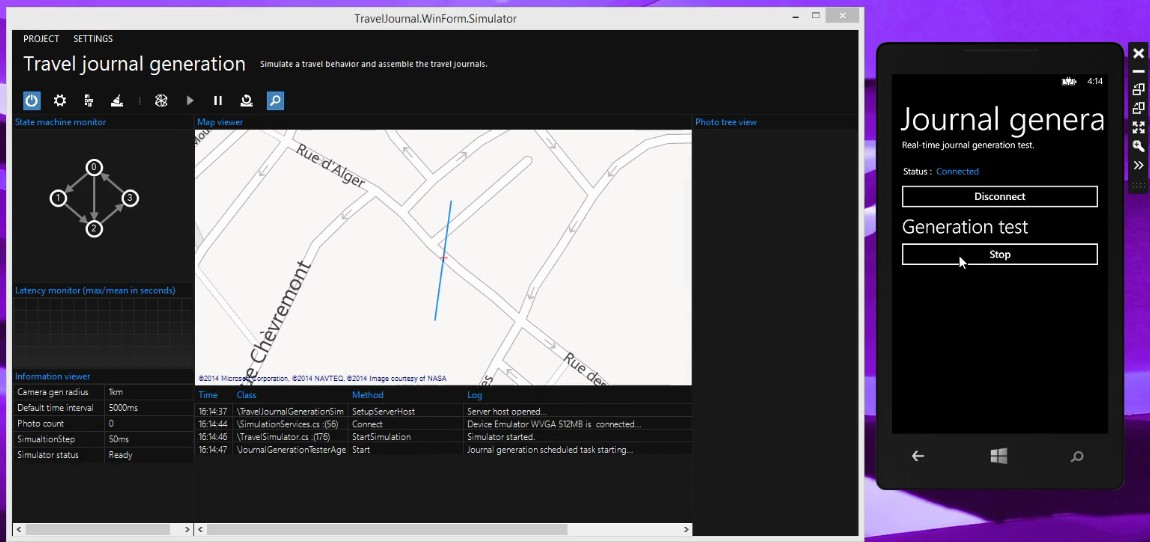
\includegraphics[width=150mm]{SIMU1.jpg}
\caption{Simulation de voyage: état initial}
\end{figure}
\ \\Lors les photos sont générés, le programme tourne à l'état 2: traitement de photo. Nous pouvons observer les itinéraire de voyage ainsi que la route parcourue. Les procédures (obtention de la position d'utilisateur, enquête de position géographique... ) de traitement sont affichées  dans le moniteur des logs.
\begin{figure}[h!]
\centering
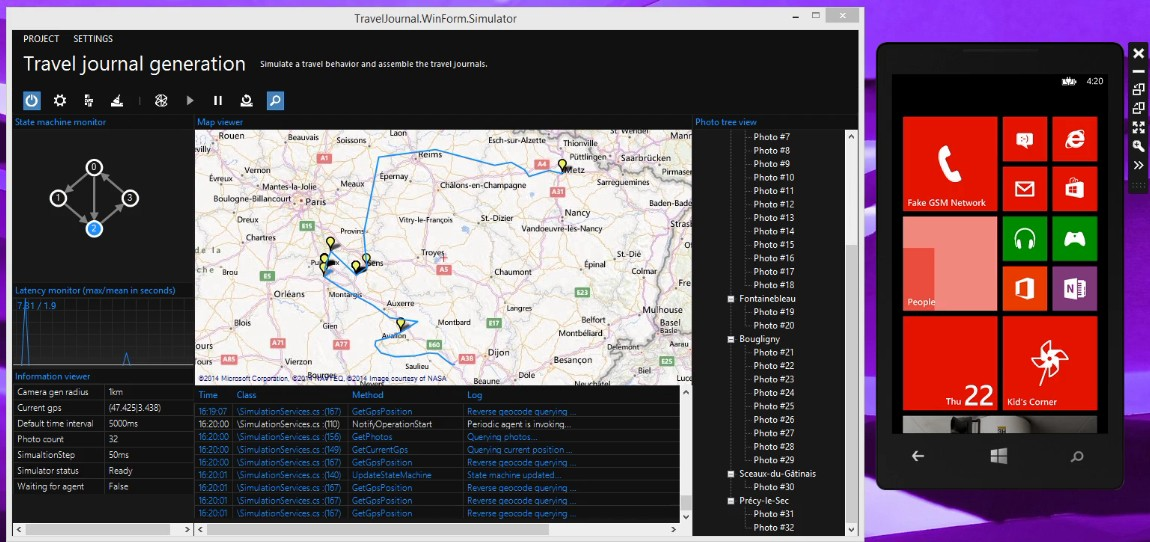
\includegraphics[width=150mm]{SIMU2.jpg}
\caption{Simulation de voyage: état de traitement des photos}
\end{figure}
\ \\A la fin, des que le curseur est retourné à Metz, l'album est complété. Un notification est envoyé à l'utilisateur pour indiquer la génération d'album.  En cliquant sur le toast de notification, l'application est ouverte est l'utilisateur peut soit partager les photos de voyage en réseau sociaux, soit les visualiser dans l'application. L'effet visuel d'interface est donné dans la section 7.
\begin{figure}[h!]
\centering
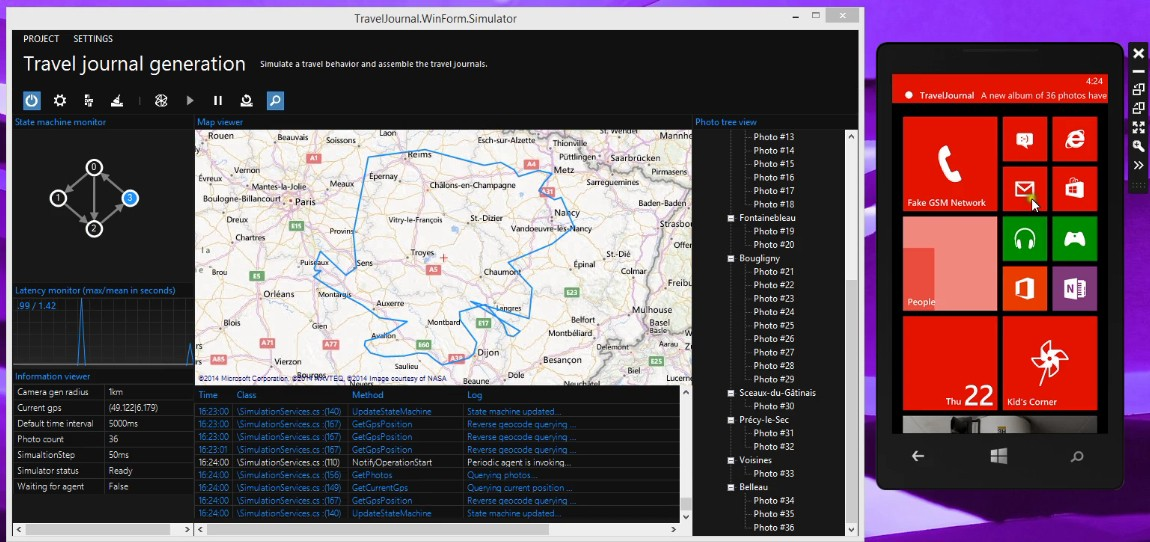
\includegraphics[width=150mm]{SIMU3.jpg}
\caption{Simulation de voyage: état de génération d'album}
\end{figure}

%----------------------------------------------------------------------------------------
% SECTION 8
%----------------------------------------------------------------------------------------
\newpage
\section{\LARGE EVOLUTION FUTURES }

A cause de la durée courte de projet, il existe encore plusieurs fonctionnements et optimisations que nous avons pas pu réalisés. Nous citons ici quelques évolutions possibles pour la commercialisation finale de notre application.
 
\vspace{0.2 cm}
\subsection{\Large Classification des photos avec les critères différentes}
Dans certaines conditions la classification des photos par l'enquête géocode n'est plus valable. Par exemple, lorsque l'utilisateur n'a pas de connexion d'internet, le lieu de voyage n'est pas reconnu (ou imprécis ) par la service (forêt, désert, etc.). Dans ce cas, une classification par les coordonnées GPS devient importante et efficace. Pour le faire, nous pouvons utiliser les algorithmes de classification comme K-moyens.

\vspace{0.2 cm}
\subsection{\Large Amélioration d'interface graphique}
Car la visualisation est très importante dans l'application, nous pensons à améliorer l'interface par les animations et les effets visuels. En inspirant de la style Suisse (\textbf{Swiss Style}), nous proposons quelques designs suivants:
   
\begin{figure}[h!]
\centering
\begin{subfigure}{.3\textwidth}
  \centering
  
\includegraphics[width=.8\linewidth]{SWISS.png}
\end{subfigure}%
\begin{subfigure}{.3\textwidth}
  \centering
  
\includegraphics[width=.9\linewidth]{SWISS2.jpg}
\end{subfigure}
\begin{subfigure}{.3\textwidth}
  \centering
  
\includegraphics[width=1\linewidth]{SWISS3.jpg}
\end{subfigure}
  \caption{Swiss Style visualisation}
\end{figure}

\ \\Quand un changement de location de ville ou de pays a lieu, un pop-up peut être affiché pour indiquer la location de ville ou de pays.

\newpage
\begin{figure}[h!]
\centering
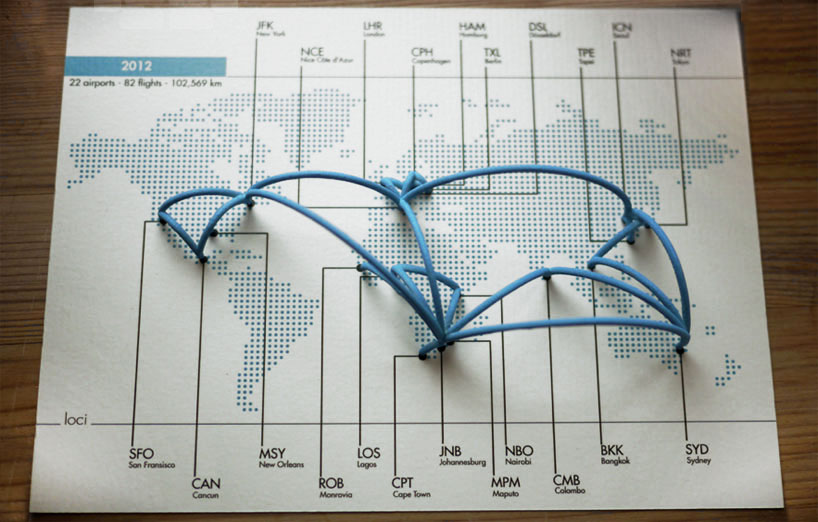
\includegraphics[width=100mm]{TRAVEL.png}
\captionof{figure}{Animation de voyage}
\end{figure}

\ \\Lors la visualisation de voyage sur la carte, une animation peut créer pour donner une dynamique sur la présentation. La moyenne de transport peut être interpréter par un calcul de vitesse (avec les données GPS), qui est ensuite visualisé dans l'animation.

\vspace{0.2 cm}
\subsection{\Large Réingénierie logicielle}
En analysant la qualité métrique de codes avec l'IDE, nous apercevons que la maintenabilité peut encore être modifiée avec la réingénierie logicielle (\textbf{Refactoring}).  Par exemple, la \textbf{complexité cyclomatique} et le \textbf{couplage des classes} peuvent être améliorés avec les patrons de conception et les réingénierie d'architecture. 

\begin{figure}[h!]
\centering
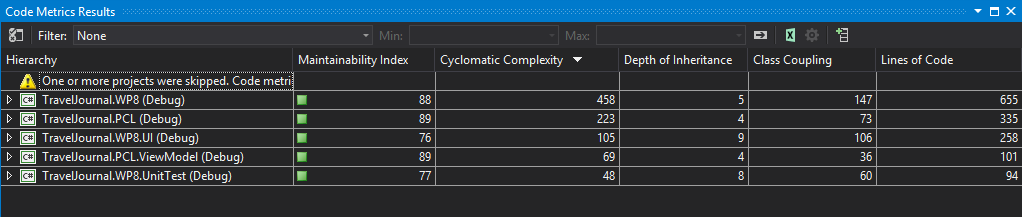
\includegraphics[width=150mm]{CODE.png}
\captionof{figure}{Analyse métrique de codes}
\end{figure}


\newpage
\subsection{\Large Optimisation de performance}
Une analyse de performance est faite pour les améliorations ultérieures. L'analyse est faite par l'IDE avec le fonctionnement  \textbf{Windows Phone Application Analysis}. Globalement la défaut plus important de l'application est le délai de l'interface utilisateur. 
\begin{figure}[h!]
\centering
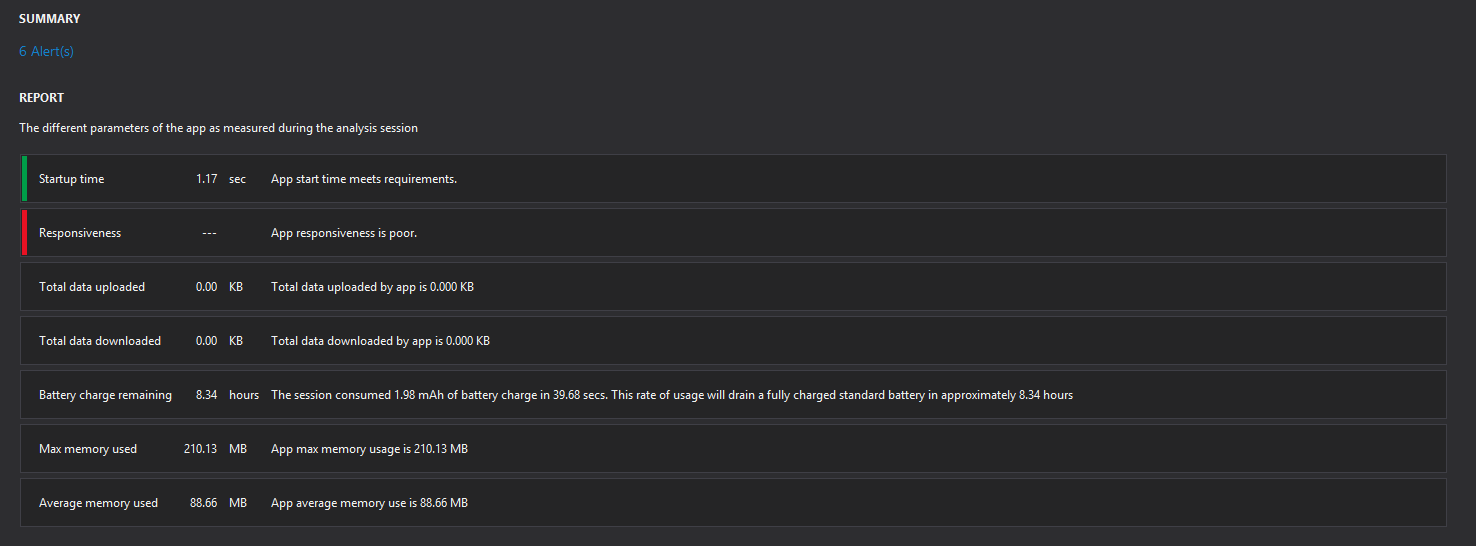
\includegraphics[width=150mm]{ANALYSE1.png}
\caption{Analyse globale de l'application}
\end{figure}
En analysant les détaillés de l'exécution, nous apercevons que ce problème devient particulièrement gênant pendant la visualisation des photos en liste ou dans la carte. Nous pensons à faire les caches de toutes les images dans le fond quand l'utilisateur ouvrir un album (\textbf{Prefetching}). Cette cache ne sera pas être très grande car seulement les imagettes seront utilisées dans les contrôles. 
\begin{figure}[h!]
\centering
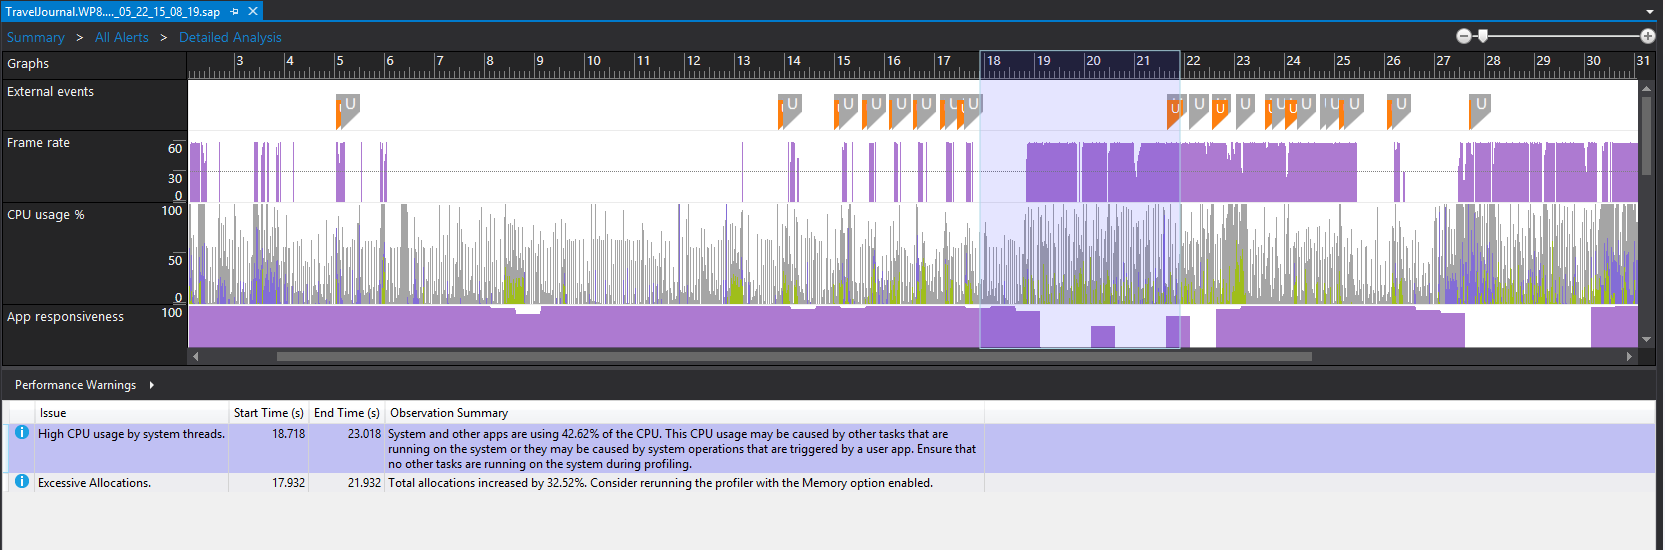
\includegraphics[width=150mm]{ANALYSE2.png}
\caption{Analyse détaille de l'exécution}
\end{figure}

%----------------------------------------------------------------------------------------
% SECTION 9
%----------------------------------------------------------------------------------------
\newpage
\section{\LARGE CONCLUSION }

Grâce à ce projet, nous avons pu expérimenter la cycle de développement complet: l'analyse de besoin et de marketing, la construction de cahier des charges, le design de l'architecture, l'implémentation, les tests et simulations. 
\\\\
De plus, nous avons pu nous familiariser avec le plate-forme Windows Phone 8. Nous avons appris plusieurs contrôles importants comme le contrôle de la carte, le contrôle Panorama, le système de navigation, etc.
\\\\
Nous avons aussi utilisé l'agent du fond (Background agent). Cette conception est fondamentale de notre système --- rien ne marche si nous ne pouvons pas encadrer les processus dans cet agent. Comme l'agent ne fonctionne que pour 25 seconds et les ressources allouées sont assez limitée, nous avons modifié plusieurs fois l'algorithme pour pouvoir obtenir un résultat satisfaisant. 
\\\\
Le simulateur joue  un rôle important dans le projet. Nous analysons la condition de simulation ainsi que la faisabilité de chaque design. Puis nous utilisons la méthodologie de développement rapide (Rapid Applciation Development ) pour créer le simulateur.  Nous partageons les tâches alors le projet avance bien pendant et après la réalisation de simulateur.
\\\\
Pendant le design et la réalisation, nous avons rencontré plusieurs difficultés concernant les choix de technologies, l'implémentation et debug, ainsi que les test et simulation. Par exemple, la connexion entre le simulateur et l'application. A cause du "sand-box" des applications, nous avons eu une difficulté pour partager les données entre l'application de Test et l'application principale. Enfin, nous avons la contourner en réalisant la synchronisation des données sur le Cloud. Ceci est aussi important pour pourvoir utiliser l'application en plusieurs équipements. Grâce à ce projet, nous avons pu nous entraîner à faire les choix techniques et décisifs en face des problèmes et difficultés.
\\\\
Nous bénéficions beaucoup des conseils de notre tuteur dans les aspects d'utilisateur et algorithmiques. Par exemple, l'idée de "préfetching"  des imagettes pour l'amélioration de performance dans l'interface d'utilisateur. Malheureusement, limité en temps, nous n'avons pas pu réaliser toutes les idées intéressantes comme le regroupement par les critères différents. Cependant elles sont intéressantes pour les versions futures.
\\\\
La recherche d'information est aussi une démarche très important pendant la réalisation. Dans le plupart du temps, nous nous référençons vers les sites informatiques comme StackOverlow et MSDN. Une recherche précise et efficace est indispensable pour la résolution des problèmes.  Par ailleurs, nous lirons aussi plusieurs œuvres classiques comme "Windows Phone 8 Receipes" pour se familiariser avec Windows phone. 
\\\\
A la fin, nous pouvons dire que ce projet a été effectué avec succès: nous avons réalise un prototype stable; nous avons construit un infrastructure efficace pour les simulations ultérieures; nous avons respecté le cahiers des charges; et enfin, nous somme pas loin à donner une version officielle pour la commercialisation.

\newpage
\section{\LARGE ANNEXE }

\vspace{0.2 cm}
\subsection{\Large Transition entre les états du traitement}

\begin{lstlisting}[label=Transition entre les états,caption=Transition entre les états]

 public class Transition
    {
        public void Transform(Processor processor)
        {
            if (processor.State == null)
            {
                throw new MissingMemberException("State not loaded");
            }
            string stateType = processor.State.GetType().Name;
            processor.UserPosition = processor.WebService.GetUserPosition().Result;
            bool haveNewPhoto = processor.PhotoManager.CheckRawPhoto(processor.Album.TimeTag);
            if (processor.UserPosition.City == processor.DataManager.Data.UserInfo.OriginalPosition.City)
            {
                if (stateType.ToUpper() == "PILOTSTATE")
                {
                    if (haveNewPhoto == false)
                    {
                        processor.State = new OriginalState();
                    }
                    else
                    {
                        processor.State = new PhotoHandlerState();
                    }
                }
                if (stateType.ToUpper() == "PHOTOHANDLERSTATE" && (!haveNewPhoto))
                {
                    processor.State = new AlbumGeneratorState();
                }
                if (stateType.ToUpper() == "ALBUMGENERATORSTATE" && processor.AlbumCompleted)
                {
                    processor.State = new OriginalState();
                }
            }
            else
            {
                if (stateType.ToUpper() == "ORIGINALSTATE")
                {
                    if (haveNewPhoto)
                    {
                        processor.State = new PhotoHandlerState();
                    }
                    else
                    {
                        processor.State = new PilotState();
                    }
                }
                if (stateType.ToUpper() == "PILOTSTATE")
                {
                    if (haveNewPhoto)
                    {
                        processor.State = new PhotoHandlerState();
                    }
                }
            }
        }
    }
\end{lstlisting}

\vspace{0.2 cm}
\subsection{\Large Traitements pour chaque état}

\begin{lstlisting}[label=Traitements pour chaque état,caption=Traitements pour chaque état]

    [DataContract]
    [KnownType(typeof(OriginalState))]
    [KnownType(typeof(PilotState))]
    [KnownType(typeof(PhotoHandlerState))]
    [KnownType(typeof(AlbumGeneratorState))]
    public abstract class State
    {
        public abstract void Execute(Processor processor);
    }
    public class OriginalState : State
    {
        public override void Execute(Processor processor)
        {

        }
    }
    public class PilotState : State
    {
        public override void Execute(Processor processor)
        {
            processor.TourRoutePoints.Add(processor.UserPosition);
        }
    }
    public class PhotoHandlerState : State
    {
        public override void Execute(Processor processor)
        {
            processor.TourRoutePoints.Add(processor.UserPosition);
            if(processor.PhotoManager.CheckRawPhoto(processor.Album.TimeTag)) 
                processor.PhotoManager.ProceedRawPhoto(processor.Album.TimeTag, processor.PhotoHandler);
        }
    }
    public class AlbumGeneratorState : State
    {
        public override async void Execute(Processor processor)
        {
            foreach (Photo p in processor.Album.PhotoList)
            {
                if (!processor.TouristCity.Contains(p.Position.City))
                    processor.TouristCity.Add(p.Position.City);
            }
            foreach (GpsPosition p in new List<GpsPosition>(processor.TourRoutePoints))
            {
                if (!processor.TouristCity.Contains(p.City))
                    processor.TourRoutePoints.Remove(p);
            }
            // Notify album completes
            processor.AlbumCompleted = true;
            processor.AlbumCompletedCallback.Invoke(processor);
        }
    }
\end{lstlisting}

%------------------------------
% END
%------------------------------
\end{document}